% !TeX program = lualatex
\documentclass{article}
\usepackage{tcolorbox}
\usepackage{ntheorem}
\usepackage{amsmath}
\usepackage{amssymb}
\usepackage{ulem}
\usepackage{graphicx}
\usepackage{centernot}
\usepackage{pgfplots}
\usepackage{tikz}
\usepackage{tikz-cd}
\usepackage{tabularx}
\usepackage{makecell}
\usepackage{mathtools}
\usepackage{emoji}
\usepackage[hidelinks, linktocpage]{hyperref}
\hypersetup{
    linktoc=all,
}
\usepackage{listings}
\usepackage[toc,page]{appendix}
\usepackage[margin=1in]{geometry}
\usepackage[parfill]{parskip}
\usepackage{nicematrix}
\usepackage{xcolor}

\definecolor{codegreen}{rgb}{0,0.6,0}
\definecolor{codegray}{rgb}{0.5,0.5,0.5}
\definecolor{codepurple}{rgb}{0.58,0,0.82}
\definecolor{backcolour}{rgb}{0.95,0.95,0.92}

\lstdefinestyle{mystyle}{
    commentstyle=\color{codegreen},
    keywordstyle=\color{magenta},
    numberstyle=\tiny\color{codegray},
    stringstyle=\color{codepurple},
    basicstyle=\ttfamily\footnotesize,
    breakatwhitespace=false,         
    breaklines=true,                 
    captionpos=b,                    
    keepspaces=true,                 
    numbers=left,                    
    numbersep=5pt,                  
    showspaces=false,                
    showstringspaces=false,
    showtabs=false,                  
    tabsize=2
}

\lstset{style=mystyle}


\everymath{\displaystyle}

\makeatletter
\newtheoremstyle{MyNonumberplain}%
  {\item[\theorem@headerfont\hskip\labelsep ##1\theorem@separator]}%
  {\item[\theorem@headerfont\hskip\labelsep ##3\theorem@separator]}%
\makeatother
\theoremstyle{MyNonumberplain}
\theorembodyfont{\upshape}

\theoremstyle{break}
\newtheorem*{proof}{Proof. }

\newcommand{\R}{\mathbb{R}}
\newcommand{\Q}{\mathbb{Q}}
\newcommand{\Z}{\mathbb{Z}}
\newcommand{\N}{\mathbb{N}}
\newcommand{\C}{\mathbb{C}}
\newcommand{\nin}{\not\in}
\newcommand{\p}{\phi}
\newcommand{\ve}{\varepsilon}
\newcommand{\ev}{\mathbb{E}}
\newcommand{\var}{\text{Var}}
\newcommand{\cov}{\text{Cov}}
\newcommand{\T}{^\intercal}
\newcommand{\der}{\operatorname{d\!}{}}
\newcommand{\evd}{\ev_{\mathcal{D}}}
\newcommand{\D}{\mathcal{D}}
\newcommand{\bias}{\text{Bias}}
\newcommand{\bt}[1]{\beta_{#1}}
\newcommand\ddfrac[2]{\frac{\displaystyle #1}{\displaystyle #2}}
\newcommand{\matindex}[1]{\mbox{\scriptsize#1}}% Matrix index
\newcommand{\inv}{^{-1}}
\newcommand{\pd}[2]{\frac{\partial {#1}}{\partial {#2}}}
\newcommand{\tr}{\text{tr}}
\newcommand{\dd}{\mathrm{d}}

\newtcolorbox{prfbox}{colback=gray!10,colframe=black!70,boxrule=0pt,arc=0pt,boxsep=2pt,left=2pt,right=2pt,leftrule=0pt}
\newtcolorbox{thmbox}{colback=orange!25,colframe=orange!85,boxrule=0pt,arc=0pt,boxsep=2pt,left=2pt,right=2pt,leftrule=2.5pt}
\newtcolorbox{defbox}{colback=blue!5,colframe=blue!70,boxrule=0pt,arc=0pt,boxsep=2pt,left=2pt,right=2pt,leftrule=2.5pt}
\newtcolorbox{ansbox}{colback=gray!10,colframe=black!70,boxrule=0pt,arc=0pt,boxsep=2pt,left=2pt,right=2pt,leftrule=0pt}
\newtcolorbox{expbox}{colback=green!10,colframe=green!70,boxrule=0pt,arc=0pt,boxsep=2pt,left=2pt,right=2pt,leftrule=2.5pt}
\newtcolorbox{warnbox}{colback=red!15,colframe=red!70,boxrule=0pt,arc=0pt,boxsep=2pt,left=2pt,right=2pt,leftrule=2.5pt}
\newtcolorbox{notebox}{colback=magenta!15,colframe=magenta!70,boxrule=0pt,arc=0pt,boxsep=2pt,left=2pt,right=2pt,leftrule=2.5pt}

\newtheorem{warning}{Warning}[section]
\newtheorem{remark}{Remark}[section]
\theoremstyle{break}
\newtheorem{theorem}{Theorem}[section]
\newtheorem{corollary}{Corollary}[theorem]
\newtheorem{proposition}{Proposition}[section]
\newtheorem{example}{Example}[section]
\newtheorem{lemma}[theorem]{Lemma}
\newtheorem{note}{Note}
\newtheorem*{question}{Question}
\newtheorem*{answer}{Answer}
\newtheorem{definition}{Definition}[section]

\renewcommand{\thempfootnote}{\textbf{\textcolor{red}\arabic{mpfootnote}}}

\title{MATH4432 Notes}
\author{SmokingPuddle58}

\begin{document}

\maketitle

\begin{center}
    This work is licensed under CC BY-NC-SA 4.0
\end{center}


\newpage

    This is the lecture note typed by SmokingPuddle in September, 2024. It mainly contains what professor mentions starting from year 3. For the contents of the first two weeks, I will try my best to include as much as possible. 

    The main reference source comes from the professor himself, lecture notes, tutorial notes, and also from the Internet if necessary.

    Please inform me if there is any errors, better within the semester or I will have a very high chance of forgetting the contents. 

    \bigskip


\begin{thmbox}
    Theorems, Corollary, Lemma, Proposition
\end{thmbox}

\begin{defbox}
    Definitions
\end{defbox}

\begin{expbox}
    Examples
\end{expbox}

\begin{warnbox}
    Warnings / Remarks
\end{warnbox}

\begin{prfbox}
    Proofs, Answers
\end{prfbox}

\begin{notebox}
    Notes
\end{notebox}

\begin{tabular}{ll}
    &\\
\end{tabular}

Some special symbols, notations and functions that will appear in this note:\bigskip

\begin{center}

    \begin{tabular}{|l|l|}
        \hline
        $\C$ & Set of complex numbers \\ \hline
        $\R$ & Set of real numbers \\ \hline
        $\Z$ & Set of integers \\ \hline
        $\Q$ & Set of rational numbers \\ \hline
    \end{tabular}
\end{center}
\begin{center}
    

\end{center}

\newpage

\tableofcontents

\newpage

% If you wish your section number begins from 1, remove / comment the line below
% \setcounter{section}{-1}

\section{Overview}

\subsection{Introduction}

Before we start, we shall clarify some of the notations that will be used.

Consider the following expression: $$P(X=x)$$

If we say $r.v.$ (Random variable) $X$, we actually means the name of the variable, while for $x$, we means the realization for such $r.v.$ 

Suppose we are now observing some quantitative response $Y$ and also input variable $X$, consisting of $p$ features, which can be expressed as:

$$
X=
    \begin{bmatrix}
        X_1 \\
        X_2 \\
        X_3 \\
        \vdots \\
        X_p
    \end{bmatrix}
$$

where $X_1,...,X_p$ are random variables. Then the relation between $Y$ and $X$ can be expressed as: 

$$
    Y=f(X)+\ve
$$

where $\ve$ is the error term independent from $X$, with mean 0, and $f$ is a deterministic function. We call such model the population level model, or ground truth model. (i.e. The number of samples is infinitely many)

\begin{warnbox}
    \begin{remark}
        Note that $Y,\ve$ are all random variables, while $X$ is a collection of random variables.
    \end{remark}
\end{warnbox}

If we want to consider a sample level (the realization of the random variables), then the equation becomes:
    \begin{eqnarray*}
             y_i= & f(x_i)+\ve_i & i=1,...,n
    \end{eqnarray*}

where $x_i$ can be a vector like the following:

$$
    x_i=
    \begin{bmatrix}
        {x_i}_1 \\
        {x_i}_2 \\
        {x_i}_3 \\
        \vdots \\
        {x_i}_p
    \end{bmatrix}
$$

and $n$ is the sample size.

\begin{warnbox}
    \begin{remark}
        In machine learning, vectors usually means \textbf{column vectors, but not row vectors}.
    \end{remark}
    For example, consider the equation $f(x)=a_1 x_1+a_2 x_2 + a_3 x_3$.
    If we know that 
    $
    a=    
    \begin{bmatrix}
        a_1 \\
        a_2 \\
        a_3
    \end{bmatrix}
    $,
        $
    x=    
    \begin{bmatrix}
        x_1 \\
        x_2 \\
        x_3
    \end{bmatrix}
    $,
    then $f(x)=a\T x$, where $a\T$ is the transpose of the vector $a$.
\end{warnbox}

Now let's go back to the ground truth model, which is $Y=f(X)+\ve$. Suppose we want to construct $f$ from the data, then we will have: 
$$
    \hat{Y}=\hat{f}(X=x)
$$

for any observed $x$.

Suppose we are interested in the difference between the data and the observed prediction, then we will be interested in the value of $\ev(Y-\hat{Y})^2$, the expected square error.

\begin{warnbox}
    \begin{remark}
        Both $Y$ and $\hat{Y}$ are random variable, since $\hat{Y}$ is the prediction that is learnt from the data, and data comes from the random sample chosen from ground truth model. 
        Thus we are not interested in the value of $(Y-\hat{Y})^2$, since it is not fixed.
    \end{remark}
\end{warnbox}

\begin{thmbox}
    \begin{theorem}
    \begin{eqnarray*}
        \ev(Y-\hat{Y})^2 & = & \underbrace{\ev(f(X)-\hat{f}(X))^2}_{\text{Reducible}} \text{ } + \underbrace{\text{ Var}(\ve)}_{\text{Irreducible}}
    \end{eqnarray*}
    \end{theorem}
    \begin{prfbox}
        \begin{proof}
            \begin{eqnarray*}
                \ev(Y-\hat{Y})^2 & = & \ev(f(X)+\ve-\hat{f}(X))^2 \\
                                 & = & \ev(f(X)-\hat{f}(X)+\ve)^2 \\
                                 & = & \ev((f(X)-\hat{f}(X))^2+2\ve(f(X)-\hat{f}(X))+\ve^2) \\
                                 & = & \ev((f(X)-\hat{f}(X))^2)+\ev(2\ve(f(X)-\hat{f}(X)))+\ev(\ve^2) \\
                                 & = & \ev((f(X)-\hat{f}(X))^2)+\underbrace{\ev(2\ve)\ev((f(X)-\hat{f}(X)))}_{\substack{\text{Assume }\ve \text{ independent from } \\ f,\hat{f}}}+\ev(\ve^2) \\
                                 & = & \ev(f(X)-\hat{f}(X))^2+\underbrace{0}_{\substack{\ev(\ve)=0}}+\ev(\ve^2) 
            \end{eqnarray*}
            Since for any random variable $X$, and its expected value, $E(X)=\mu$, we have: (Covered in MATH2411)
            \begin{eqnarray*}
                \text{Var}(X) & = & \ev(X-\mu)^2\\
                              & = & \ev(X^2)+\ev(\mu^2)-2\ev(X\mu)\\
                              & = & \ev(X^2)+\mu^2-2\mu\ev(X)\\
                              & = & \ev(X^2)+\mu^2-2\mu^2\\
                              & = & \ev(X^2)-\mu^2
            \end{eqnarray*}
            Thus, 
            \begin{eqnarray*}
                \ev(Y-\hat{Y})^2 & = & \ev(f(X)-\hat{f}(X))^2+\ev(\ve^2) \\
                                 & = & \ev(f(X)-\hat{f}(X))^2+\var(\ve)
            \end{eqnarray*}
        \end{proof}
    \end{prfbox}
\end{thmbox}

To conclude, you can only reduce the error for the reducible part, by making your model approximate the ground truth model as well as possible, 
while we can really do not much on the irreducible part.

\subsection{Estimation of $f$}

There are two methods for estimating $f$, namely parametric, and non-parametric methods.

For parametric method, we assume that $f$ can be described by a set of parameters, such that once all of the parameters are known, then the model is known.

\begin{expbox}
    \begin{example}
        One of the most simple assumption is that $f$ is linear in $X$, which can be described as:  $$f(X)=\beta_0+\beta_1X_1+\beta_2X_2+...+\beta_pX_p$$
    \end{example}
\end{expbox}

For non-parametric method, we do not pre-specify the form of the model (Can be linear, non-linear. tree and neural network). To 
control the flexibility, we can always tune the parameters.

The advantages and disadvantages are listed in the following table.

\begin{table}[!h]
    \centering
    \begin{tabular}{|l|l|l|}
    \hline
                    & Parametric                                       & Non-parametric                                          \\ \hline
    Advantage    & Easy to solve and understand                     & More flexible and sometimes more powerful               \\ \hline
    Disadvantage & \makecell{The model may be too simple\\ to fit into the data} & \makecell{The model may be too flexible, \\there may be overfitting} \\ \hline
    \end{tabular}
\end{table}

\begin{center}
    \includegraphics*[scale=0.35]{Images/img1.png}
\end{center}

\begin{table}[!h]
    \centering
    \begin{tabular}{|l|l|}
    \hline
    Ground truth model & Underfitting                         \\ \hline
    Good estimation    & Overfitting (Fitting into the noise) \\ \hline
    \end{tabular}
\end{table}

The above image shows the example of a ground truth model, a good estimation, overfitting and underfitting. It is also included in the lecture 
note. 

\subsection{Assessing Model Accuracy}

In statistical machine learning context, to find a good estimate $f$, we shall introduce the concept of regularization 
(Covered in detail later), in which we want to minimize the following value as much as possible:
$$\text{Loss}(Y,f)+\lambda R(f)$$
where $Y$ is the response, $\lambda$ is a tuning parameter (weight) for the regularizer $R(f)$ of the model $f$.

The introduction of the regularizer is trying to control the complexity / flexibility of the function $f$ to prevent perfect fit / overfitting issue.

\begin{expbox}
    \begin{example}[Spline interpolation]
        Consider the loss function and the regularizer as: $$\underbrace{\sum_{i=1}^{n_{\text{train}}}(y_i-g(x_i))^2}_{\text{Loss function}}+\lambda\underbrace{\int g''(t)^2\der t}_{\text{Regularizer}}$$
        \medskip
        The regularizer tries to control the second derivative of $g$ to be as small as possible to ensure smoothness.
        
        Assume that $\lambda$ is a extremely large value, the only solution is to let the integral to be 0, i.e. $g(t)$ should 
        be a linear function.
        \medskip

        If we put $\lambda=0$, then the solution will be $$\hat{g}(x_i)=y_i$$

        i.e. The model will have a perfect fit to the data.
        \medskip

        If we tune the parameter correctly, then we can get a good model that is neither overfit nor underfit.
    \end{example}
\end{expbox}

So how do we know if our tuning parameter is good or not?

Consider there is a set of data $\{(x_i,y_i)\}_{i=1...n}$, and we want to minimize $$\sum_{i=1}^{n}(y_i-g(x_i))^2+\lambda R(f)$$ as much as possible.

To achieve that, we need to spilt the data into two parts: Training data and Testing data, and the two set of datasets
should not be overlapping with each other.

The idea is, we only use the training data for solving optimization. After such process, we will 
obtain $\hat{g}$, which is estimated from the training data. The testing data is then used to evaluate whether the model is accurate or not. i.e. We would like to 
evaluate the value of $$\frac{1}{n}\sum_{i=1}^{n}(y_i-\hat{g}(x_i))^2$$
where $n$ is the number of testing data. Such value is defined as MSE (Mean Square Error).

\begin{defbox}
    \begin{definition}[Mean Square Error]
        $$MSE=\frac{1}{n}\sum_{i=1}^{n}(y_i-\hat{g}(x_i))^2$$ where $g(x_i)$ is 
        the prediction $\hat{g}$ gives for the $i-$th prediction.
    \end{definition}
\end{defbox}

\begin{center}
    \includegraphics*[scale=0.35]{Images/img2.png}
\end{center}

\begin{table}[!h]
    \centering
    \begin{tabular}{|l|l|}
    \hline
    Black: Ground truth model & Red: Testing error                         \\ \hline
    Yellow: Simple linear model    & Gray: Training error \\ \hline
    Green: Perfect model (Fit all data into the model)    &  \\ \hline
    \end{tabular}
\end{table}

In the red curve, there are three point corresponding to the three different models on the left, which shows the MSE of overfitting
, underfitting and a good model. 

\begin{defbox}
    \begin{definition}[Training and Testing Error]
        Suppose $\hat{g}_\lambda$ is estimated from the data, and depends on $\lambda$, then the accuracy of $\hat{g}_\lambda$ based on the testing data is given by:
        $$\frac{1}{n_\text{Test}}\sum_{i\in\text{Test}}(y_i-\hat{g}_\lambda(x_i))^2$$
        This is called \textbf{testing mean square error (TMSE)}.

        \bigskip
        The \textbf{training error} is given by: $$\frac{1}{n_\text{Train}}\sum_{i\in\text{Train}}(y_i-\hat{g}_\lambda(x_i))^2$$
    \end{definition}
\end{defbox}

\begin{notebox}
    \begin{note}
        Training error is usually less than testing error, since optimization is solved with testing error, especially when you put $\lambda=0$.
    \end{note}
\end{notebox}

\begin{center}
    \includegraphics*[scale=0.35]{Images/img3.png}
\end{center}

Note that linear regression above provides a very poor fit to the data, while perfect fit model 
does not increase error too much, since the noise is very small. 

\begin{center}
    \includegraphics*[scale=0.35]{Images/img4.png}
\end{center}

For this dataset, the ground truth model is close to linear, and due to the large noise,
the high flexibility gives more error.

\newpage

\subsection{Bias-Variance Trade-Off}

As shown in the previous example, we can see that the testing error are in U-shape. To understand
the reason, we will need to introduce the concept of bias-variance trade-off.

Suppose we are interested in learning an unknown function $f(X)$ from the dataset $\mathcal{D}$,
namely $\hat{f}(X;\mathcal{D})$. Then at some future query point $X=x_0$, we want to
find $\hat{f}$, such that $\hat{f}$ satisfies: $$\min_{\hat{f}}[f(x_0)-\hat{f}(x_0;\mathcal{D})|X=x_0]^2$$

However are we really interested in evaluating this? Actually No! It is because the 
training dataset comes from a random selection! The prediction may not be accurate
if we changed another training dataset.

In order to solve the problem, we should take the random selection process in an \textbf{average sense}. 

Thus we are actually more interested in the following: $$\min_{\hat{f}}\evd[f(x_0)-\hat{f}(x_0;\mathcal{D})|X=x_0]^2$$

\begin{thmbox}
    \begin{theorem}
        \begin{eqnarray*}
            \evd[f(x_0)-\hat{f}(x_0;\mathcal{D})|X=x_0]^2&=&\underbrace{[f(x_0)-\evd(\hat{f}(x_0;\mathcal{D}))|X=x_0]^2}_{\text{Bias}^2}\\
            &+&\underbrace{\evd[[\evd(\hat{f}(x_0;\mathcal{D}))-\hat{f}(x_0;\mathcal{D})|X=x_0]^2]}_{\text{Variance}}
        \end{eqnarray*}
    \end{theorem}
    \begin{prfbox}
        \begin{proof}
            \begin{eqnarray*}
                [f(x_0)-\hat{f}(x_0,\mathcal{D})|X=x_0]^2 & = & [f(x_0)\underbrace{-\evd(\hat{f}(x_0;\mathcal{D}))+\evd(\hat{f}(x_0;\mathcal{D}))}_{=0}-\hat{f}(x_0,\mathcal{D})|X=x_0]^2\\
                &=& [f(x_0)-\evd(\hat{f}(x_0;\mathcal{D}))|X=x_0]^2 + [\evd(\hat{f}(x_0;\mathcal{D}))-\hat{f}(x_0,\mathcal{D})|X=x_0]^2\\
                &+& 2[f(x_0)-\evd(\hat{f}(x_0;\mathcal{D}))|X=x_0][\evd(\hat{f}(x_0;\mathcal{D}))-\hat{f}(x_0,\mathcal{D})|X=x_0]
            \end{eqnarray*}

            Now we take expectation to the expression above with respect to $\mathcal{D}$. We have:
            \begin{eqnarray*}
                &   &\evd[f(x_0)-\hat{f}(x_0,\mathcal{D})|X=x_0]^2\\
                & = & \underbrace{[f(x_0)-\evd(\hat{f}(x_0;\mathcal{D}))|X=x_0]^2}_{\text{Bias, as constant value}}\\
                & + & \underbrace{\evd\biggl([\evd(\hat{f}(x_0;\mathcal{D}))-\hat{f}(x_0,\mathcal{D})|X=x_0]^2\biggr)}_{\text{Variance}}\\
                & + & 2 \evd \biggl\{[f(x_0)-\evd(\hat{f}(x_0;\mathcal{D}))|X=x_0][\evd(\hat{f}(x_0;\mathcal{D}))-\hat{f}(x_0,\mathcal{D})|X=x_0]\biggr\}
            \end{eqnarray*}
            Consider the last term, we expand this term, then we will have: 
                \begin{eqnarray*}
                    && 2 \evd \biggl\{[f(x_0)-\evd(\hat{f}(x_0;\mathcal{D}))|X=x_0][\evd(\hat{f}(x_0;\mathcal{D}))-\hat{f}(x_0,\mathcal{D})|X=x_0]\biggr\} \\
                \end{eqnarray*}
        \end{proof}
    \end{prfbox}
\end{thmbox}

\begin{thmbox}
    \begin{prfbox}
        \begin{eqnarray*}
            &=& 2 \evd \biggl\{f(x_0)\evd[\hat{f}(x_0;\mathcal{D})]-f(x_0)\hat{f}(x_0;\mathcal{D})-[\evd[\hat{f}(x_0;\mathcal{D})]]^2+\hat{f}(x_0;\mathcal{D})\evd[\hat{f}(x_0;\mathcal{D})]\biggr\} \\
            &=& 2  \textcolor{red}{\biggl\{}\evd\biggl\{f(x_0)\evd[\hat{f}(x_0;\mathcal{D})]\biggr\}-\evd\biggl\{f(x_0)\hat{f}(x_0;\mathcal{D})\biggr\}-\evd\biggl\{[\evd[\hat{f}(x_0;\mathcal{D})]]^2\Biggr\} \\
            &+& \evd\biggl\{\hat{f}(x_0;\mathcal{D})\evd[\hat{f}(x_0;\mathcal{D})]\biggr\}\textcolor{red}{\Biggr\}}\\
            &=& \evd(f(x_0))\evd(\hat{f}(x_0;\mathcal{D}))-\evd(f(x_0))\evd(\hat{f}(x_0;\mathcal{D}))-\evd(\hat{f}(x_0;\mathcal{D}))^2+\evd(\hat{f}(x_0;\mathcal{D}))^2\\
            &=& 0
        \end{eqnarray*}
        The last term vanished, since we know that $\evd(f(x_0))=f(x_0)$ and $\evd(\evd(\hat{f}(x_0;\mathcal{D}))) = \evd(\hat{f}(x_0;\mathcal{D})).$

        \bigskip
        Also do note that even though $\hat{f}(X;\mathcal{D})$ is a random variable due to the randomness of the dataset, $\evd\hat{f}(X;\mathcal{D})$ is 
        no longer a random variable with respect to $\mathcal{D}$.

        \begin{expbox}
            \begin{example}
                If $Z\sim N(\mu,\sigma^2)$ is a random variable, then $\ev(Z)=\mu$ is no longer random variable.
            \end{example}
        \end{expbox}

    \end{prfbox}
\end{thmbox}
\begin{notebox}
    \begin{note}
        The reason for us to condition on $x_0$, is because we want to simplify the entire process.

        In fact, by using total expectation law, we are able to evaluate for $\evd\bigl[f(X)-\hat{f}(X;\mathcal{D})\bigr]^2$.

        \begin{thmbox}
            \begin{theorem}[Total Expectation Law]
                Given any random variables $X,Y$, then we have 
                $$\ev(X)=\ev_Y\Bigl(\ev(X|Y)\Bigr)$$ 
            \end{theorem}
        \end{thmbox}
        Thus we have: 
        \begin{eqnarray*}
            \evd\bigl[f(X)-\hat{f}(X;\mathcal{D})\bigr]^2 &=& \ev_X\biggl[\evd\bigl[f(X)-\hat{f}(X;\mathcal{D})\bigr]^2|X=x_0\biggr].
        \end{eqnarray*}
    \end{note}
\end{notebox}

\begin{notebox}
    \begin{note}
        Practically, $\evd\biggl(\hat{f}(x_0;\mathcal{D})\biggr)$ can be estimated by: 
        \begin{eqnarray*}
            \evd\biggl(\hat{f}(x_0;\mathcal{D})\biggr)&=&\frac{1}{B}\sum_{b=1}^B \hat{f}^{(b)}(x_0)
        \end{eqnarray*}
        From this, we can estimate the variance term by:
            \begin{eqnarray*}
                \evd\biggl[[\evd(\hat{f}(x_0;\mathcal{D}))-\hat{f}(x_0;\mathcal{D})|X=x_0]^2\biggr] &=& \frac{1}{B} \Biggl(\sum_{b=1}^B\biggl[\hat{f}(x_0)-\frac{1}{B}\sum_{b=1}^B\hat{f}^{(b)}(x_0)\biggr]\Biggr).
            \end{eqnarray*}

            This implies that, to estimate for variance, it is not necessary for us to know the ground-truth model. However, to know the bias, we do need to know the ground-truth model.
    \end{note}
\end{notebox}

\begin{defbox}
    \begin{definition}[Bias and Variance]
        Given an estimator $\hat{\theta}$ for some parameter $\theta$, the bias is defined as: 
        $$\text{Bias}(\hat{\theta},\theta)=\ev(\hat{\theta})-\theta$$
        while given a random variable $X$, the variance is defined as:
        $$
            \text{Var}(X)=\ev\bigl[(X-\ev(X))^2\bigr].
        $$
    \end{definition}
\end{defbox}

\begin{notebox}
    \begin{note}
        When we talk about variance here, such as $\var(\hat{\beta})$, mostly we means the variance \textbf{due to the change of the training data}.
    \end{note}
\end{notebox}

Suppose we are interested in a model that perfectly fits into the data. For example,

$$Y=f(X)+\ve$$

This is the population-level model we seen before. Let $\text{Var}(\ve)=\sigma^2$ and $\ev{(\ve)}=0$,

We now take samples from such model, we will then have $(x_i,y_i)$ that is in relationship of:
\begin{eqnarray*}
    y_i=f(x_i)+\ve_i &  & i=1,...,n
\end{eqnarray*}

We are interested in finding $g$, where $g$ can minimizes:

$$\sum_{i}(y_i-g(x_i))^2.$$

After solving the optimization problem, we will obtain $\hat{g}$, that $\hat{g}(x_i)=y_i, i=1,...,n$.

To adopt bias-variance view, we will have to evaluate $\ev(\hat{g})\text{ and Var}(\hat{g})$.

Note that:

\begin{eqnarray*}
    \ev(\hat{g}(x_i)) &=& \ev(y_i)\\
                      &=& \ev(f(x_i)+\ve_i)\\
                      &=& \ev(f(x_i))\\
                      &=& f(x_i)
\end{eqnarray*}

To see if our estimator having bias or not, we only need to check $\ev(\hat{g}(x_i))-f(x_i)$.

However, since $\ev(\hat{g}(x_i))=f(x_i)$, thus $\ev(\hat{g}(x_i))-f(x_i)=0$. This implies if the model is very flexible
that can perfectly fits into the data, then the model is unbiased. 

Now, consider the variance, we have: 
\begin{eqnarray*}
    \var(\hat{g}(x_i)) &=& \var(y_i)\\
                       &=& \var(f(x_i)+\ve_i)\\
                       &=& \var(\ve_i)\\
                       &=& \sigma^2
\end{eqnarray*}
 
For a very flexible model, the bias can be very small, while the variance will be extremely large. 

\begin{center}
    \includegraphics*[scale=0.1]{Images/img5.jpg}
\end{center}

Suppose there is an dataset $\mathcal{D}$, and we want to solve the following optimization problem: $$\min_g\sum_{i=1}^{n}\bigl((y_i-g(x_i))\bigr)^2+\lambda\cdot R(g)$$

If $g(x_i)=C$ is a constant function (That is, totally not fitting into the data).

Since $\ev(\hat{g}(x_i))=C$, and $\var(\hat{g})=0$.

Thus 
\begin{eqnarray*}
    \bias &=&\ev(\hat{g}(x_0))-f(x_0)\\
          &=& C-f(x_0).
\end{eqnarray*}

This is not reducible, which implies the model is biased. However, the variance is 0. 

To conclude, we want to find a model, which can keeps a perfect balance between bias and variance. The
model may be good, even if the model is biased.

\begin{center}
    \includegraphics*[scale=0.3]{Images/img6.png}
\end{center}

\begin{table}[!h]
    \centering
    \begin{tabular}{|l|l|l|}
    \hline
           Red line: Test MSE     & Blue line: Bias                                       & Orange line: Variance                                        \\ \hline
    \end{tabular}
\end{table}

\section{Regression analysis}
\subsection{Simple Linear Regression}
\begin{defbox}
    \begin{definition}[Simple Linear Regression]
        In simple linear regression, there are only 1 variable, and thus there is only 2 parameters to fit in, which is:
        $$Y=\underbrace{\bt{0}+\bt{1}X}_{f(X)}+\ve.$$
    \end{definition}
\end{defbox}

Suppose we want to estimate $\hat{\bt{0}},\hat{\bt{1}}$, then we have the realization value to be:

$$\hat{Y}=\bt{0}+\bt{1}X.$$

To figure out the estimate, suppose there is some observed training data $D=\biggl\{(x_i,y_i)\biggr\}_{i=1...n}$.

What we want to do now is to solve the optimization problem on the squared loss:
$$(\hat{\bt{0}},\hat{\bt{1}})=\arg\min_{\bt{0},\bt{1}}\sum_{i=1}^n\bigl(y_i-\bt{0}-\bt{1}x_i\bigr)^2.$$

This problem is also known as least square problem, and the figure below shows the function that we want to find the optimized value.

\begin{center}
    \includegraphics*[scale=0.25]{Images/img7.png}
\end{center}

\begin{thmbox}
    \begin{theorem}[Least Square Problem]
        The solution to the least square problem is given by: 
    \end{theorem}
        \begin{eqnarray*}
            \hat{\bt{1}}&=& \ddfrac{\sum_{i=1}^n(x_i-\bar{x})(y_i-\bar{y})}{\sum_{i=1}^n(x_i-\bar{x})^2}\\
            \hat{\bt{0}}&=& \bar{y}- \hat{\bt{1}}\bar{x}
        \end{eqnarray*}
        \begin{prfbox}
            \begin{proof}
                I have a proof of this theorem, but there is not enough space in this margin to write it. \emoji{nerd-face}\emoji{point-up}
            \end{proof}
        \end{prfbox}
\end{thmbox}

\begin{prfbox}
    \begin{question*}
        Given $\mathcal{D}^{(1)}$, we can generate $\hat{\bt{0}}^{(1)}$ and $\hat{\bt{1}}^{(1)}$.

        Given $\mathcal{D}^{(2)}$, we can generate $\hat{\bt{0}}^{(2)}$ and $\hat{\bt{1}}^{(2)}$.
        etc.

        In an average sense, will $\hat{\bt{0}}^{(1)}=\bt{0}^*$? i.e. does $$\evd\bigl({\bt{0}}^{(1)}\bigr)=\bt{0}^*$$

        \begin{answer}
            Unbiased
        \end{answer}
    \end{question*}

\end{prfbox}

Consider the variance of $\hat{\bt{0}},\hat{\bt{1}}$, which is $\var(\hat{\bt{0}})$ and $\var(\hat{\bt{1}})$. We always wanted to keep the variance as small as possible. The following shows an example of the estimation of $\hat{\bt{0}}$ and $\hat{\bt{1}}$. Note that both of them are unbiased, however, the one on the right hand side obviously have a larger variance than the left hand side. 

\begin{center}
    \includegraphics*[scale=0.1]{Images/img8}
\end{center}

\begin{defbox}
    \begin{definition}[Quadratic Form]
        If $A$ is a positive definite matrix, then $f$ is called a quadratic from, if:
        $$f(x)=x\T Ax$$
    \end{definition}
\end{defbox}

\begin{expbox}
    \begin{example}
        Consider the equation
        $$x_1^2+x_2^2=1.$$
        We can write this equation into quadratic form:
        $$\begin{bmatrix}
            x_1\\
            x_2
        \end{bmatrix}\T
       \begin{bmatrix}
            1 & 0\\
            0 & 1
        \end{bmatrix}
        \begin{bmatrix}
            x_1\\
            x_2
        \end{bmatrix}.
        $$
    \end{example}
\end{expbox}

With quadratic form, we can rewrite the least square problem as:

$$\sum_{i=1}^n (y_i-x_i\T\beta)^2$$.

\begin{defbox}
    \begin{definition}[Residual Sum of Square (RSS)]
        The residual sum of square is the sum of the square of the error terms. i.e.
        \begin{eqnarray*}
            RSS&=&e_1^2+e_2^2+...+e_n^2\\
               &=&\sum_{i=1}^n(y_i-\hat{\bt{0}}-\hat{\bt{1}}x_i)^2
        \end{eqnarray*}
    \end{definition}
\end{defbox}

We would like to know how accurate is our estimated parameter as estimate of ground truth value. This can be done by computing the standard error these parameters.

\begin{thmbox}
    \begin{theorem}
        Define $SE$ as standard error. We have:
        \begin{eqnarray*}
            SE(\hat{\mu})^2&=&\frac{\sigma^2}{n}\\
            SE(\hat{\bt{0}})&=&\sigma^2\Biggl[\frac{1}{n}+\frac{\bar{x}^2}{\sum_i^n (x_i-\bar{x})^2}\Biggr]\\
            SE(\hat{\bt{1}})&=&\frac{\sigma^2}{\sum_i^n (x_i-\bar{x})^2}
        \end{eqnarray*}
        where $\sigma^2$ is estimated by $\hat{\sigma}^2=\frac{RSS}{n-2}$
    \end{theorem}
\end{thmbox} 

\begin{notebox}
    \begin{note}
        The reason why the denominator for $\hat{\sigma}^2$ is $n-2$, is because we are estimating 2 parameters. This is related to degree of freedom.
        Let's take a very simple example:
        \begin{expbox}
            \begin{example}
                Let $z_i\sim N(\mu,\sigma^2)$. Suppose we pick 3 data points: $\{z_1,z_2,z_3\}$. Then we can estimate the mean by the following formula:
                $$\hat{\mu}=\frac{1}{3}(z_1+z_2+z_3).$$
                Suppose we now know the value of $z_1,z_2$ and $\hat\mu$. Then we will also know the value of $z_3$. The number of sample is no longer 3, since
                when we know 2 of them, we immediately get the third one, with the constraint of the value of $\hat\mu$.
            \end{example}
        \end{expbox}
    \end{note}
\end{notebox}

\begin{defbox}
    \begin{definition}[$t$-statistics]
        Given the null hypothesis of 
        $$\mathcal{H}_0:\bt{1}=0,$$
        $t$-statistics is defined as:
        $$t=\frac{\hat{\bt{1}}-{\bt{1}}}{SE(\hat{\bt{1}})},$$
        which we have a $t$-distribution with $n-2$ degree of freedom.

    \end{definition}
\end{defbox}

We will reject the null hypothesis if we observe a very large $|t|$, or $p$-value is small enough.

To access the accuracy of a model, we will use $R^2$. But first we shall define the residual standard error.

\begin{defbox}
    \begin{definition}[Residual Standard Error (RSE)]
        \begin{eqnarray*}
            RSE &=& \sqrt{\frac{1}{n-2}RSS}\\
                &=& \sqrt{\frac{1}{n-2}\sum_{i=1}^n (y_i-\hat{y_i}^2)} .
        \end{eqnarray*}
    \end{definition}
\end{defbox}

\begin{defbox}
    \begin{definition}[$R^2$]
        \begin{eqnarray*}
            R^2 &=& \frac{TSS-RSS}{TSS}\\
            &=& 1 - \frac{RSS}{TSS}.
        \end{eqnarray*}
        where $TSS=\sum(y_i-\bar{y})$ is the total sum of squares.
    \end{definition}
\end{defbox}

\begin{warnbox}
    \begin{remark}
        If we calculate $R^2$ based on the testing / future data, we call that predicted $R^2$.
        In such case, $R^2$ can be negative, if the method is really bad, even worse than 0.
    \end{remark}
\end{warnbox}

\begin{warnbox}
    \begin{remark}
        $R^2$ is mainly used in simple linear regression, and we seldom apply it to multivariable regression.
    \end{remark}
\end{warnbox}

\subsection{Multiple Linear Regression}

\begin{defbox}
    \begin{definition}[Multiple Linear Regression]
        In multiple linear regression, there are $p$ distinct variables, and thus there are $p$ parameters to fit in, that is:
        $$Y=\underbrace{\bt{0}+\bt{1}X_1+\bt{2}X_2+...+\bt{p}X_p}_{f(X)}+\ve.$$
    \end{definition}
\end{defbox}

\begin{thmbox}
    \begin{theorem}[Least Square Problem]
        Let $\hat\beta=[\hat\beta_{0},\hat\beta_{1},...,\hat\beta_{p}]$ be the least squares

        $$\hat\beta=\arg\min_{\beta=[\beta_{0},\beta_{1},...,\beta_{p}]}\sum_i^n(y_i-\bt{0}-\bt{1}x_{i1}-...-\bt{p}x_{ip})^2$$

        The solution to the least square problem in multple linear regression is given by: 

        $$\hat\beta=(X\T X)^{-1}X\T y.$$

        Where: 

        \begin{eqnarray*}
           y=\begin{bmatrix}
            y_1 \\
            y_2 \\
            ... \\
            y_n 
            \end{bmatrix} \text{ is the response} &\text{and}& X=
            \begin{bmatrix}
                1 & x_{11} &...& x_{1p}\\
                1 & x_{21} &...& x_{2p}\\
                ...&...&...&...\\
                1 & x_{n1} &...& x_{np}\\
            \end{bmatrix} \text{ is the design matrix.}
        \end{eqnarray*}
    \end{theorem}
        \begin{prfbox}
            \begin{proof}
                Our goal is to evaluate for:

                \begin{eqnarray}
                    \min_{\bt{0},...,\bt{p}}\sum_{i=1}^n \bigl(y_i-(\bt{1}x_{i1}+...+\bt{p}x_{ip})\bigr)^2
                \end{eqnarray}

            \end{proof}
        \end{prfbox}
\end{thmbox}


\begin{thmbox}
    \begin{prfbox}
        Define 
        $$y=
            \begin{bmatrix}
                y_1 \\
                y_2 \\
                ... \\
                y_n 
            \end{bmatrix}
            , X=
            \begin{bmatrix}
                1 & x_{11} &...& x_{1p}\\
                1 & x_{21} &...& x_{2p}\\
                ...&...&...&...\\
                1 & x_{n1} &...& x_{np}\\
            \end{bmatrix} 
            , \text{ and } \beta=
            \begin{bmatrix}
                \beta_1 \\
                \beta_2 \\
                ... \\
                \beta_p
            \end{bmatrix}.$$
    If we observe deeply \emoji{flushed}, we can see if we take $i$-th row of $(y-X\beta)$, then we will get exactly: $$(y-X\beta)_i=\bigl(y_i-(\bt{1}x_{i1}+...+\bt{p}x_{ip})\bigr).$$

    Note that for any \textbf{column vector}, say $y$, we have (Just some equivalent forms for reference)
    \begin{eqnarray*}
        \sum_{i=1}^n y_i^2 &=& y_1^2+y_2^2+...+y_n^2 \\
                           &=& y\T y\\
                           &=& \left\lVert y\right\rVert^2.
    \end{eqnarray*}
    We can now rewrite the equation (1) into the form of:
    \begin{eqnarray*}
        & & \sum_i \bigl((y-X\beta)_i\bigr)^2\\
        &=& (y-X\beta)\T (y-X\beta).
    \end{eqnarray*}
    Our goal now changes to:
    \begin{eqnarray}
        \min_\beta (y-X\beta)\T (y-X\beta).
    \end{eqnarray}
    Since:
    \begin{eqnarray*}
        & &(y-X\beta)\T (y-X\beta) \\
        &=&(y\T-\beta\T X\T) (y-X\beta)\\
        &=&y\T y - y\T X\beta - \beta\T X\T y + \beta\T X\T X\beta.
    \end{eqnarray*}
    This is in fact a quadratic form, and if we treat it as a function of $\beta$, then this is going to be a quadratic function.

    Note that $y\T X\beta$ and $\beta\T X\T y$ are actually equivalent. The reason why is because $y\T X\beta$ is actually a scalar, since the multiplication result has a dimension of
    \begin{eqnarray*}
        (1,p) \times (p,n) \times (1,n) &=& (1,n) \times (n,1)\\
                                        &=& (1,1)
    \end{eqnarray*}
    We can take transpose to a scalar without changing its value. Then $(y\T X\beta)\T = \beta\T X\T y$. Thus:
    \begin{eqnarray*}
        & &y\T y - y\T X\beta - \beta\T X\T y + \beta\T X\T X\beta\\
        &=&y\T y - 2y\T X\beta + \beta\T X\T X\beta
    \end{eqnarray*}

    Now we take derivative w.r.t. $\beta$ for $y\T y - 2y\T X\beta + \beta\T X\T X\beta$. We have:


    \end{prfbox}
\end{thmbox} 

\begin{thmbox}
    \begin{prfbox}
        \begin{eqnarray*}
            & &\frac{\partial}{\partial\beta} y\T y - 2y\T X\beta + \beta\T X\T X\beta\\
            &=& 0-2(X\T y)\T\beta+2X\T X\beta
        \end{eqnarray*}   
        Set the term to be zero, then we have:
        \begin{eqnarray}
            X\T X\beta &=& X\T y\\
            \beta &=& (X\T X)^{-1} X\T y
        \end{eqnarray}
        Note that the dimension on the L.H.S. of (3) will be $(p+1,p+1)\times(p+1,1)=(p+1,1)$. This implies there are $(p+1)$ constraints, and therefore reducing $p+1$ degree of freedoms.
    \end{prfbox}
\end{thmbox}

The geometric meaning of the solution is actually the projection onto the plane spanned by $x_1,x_2$ (Yellow Region). 
\begin{center}
    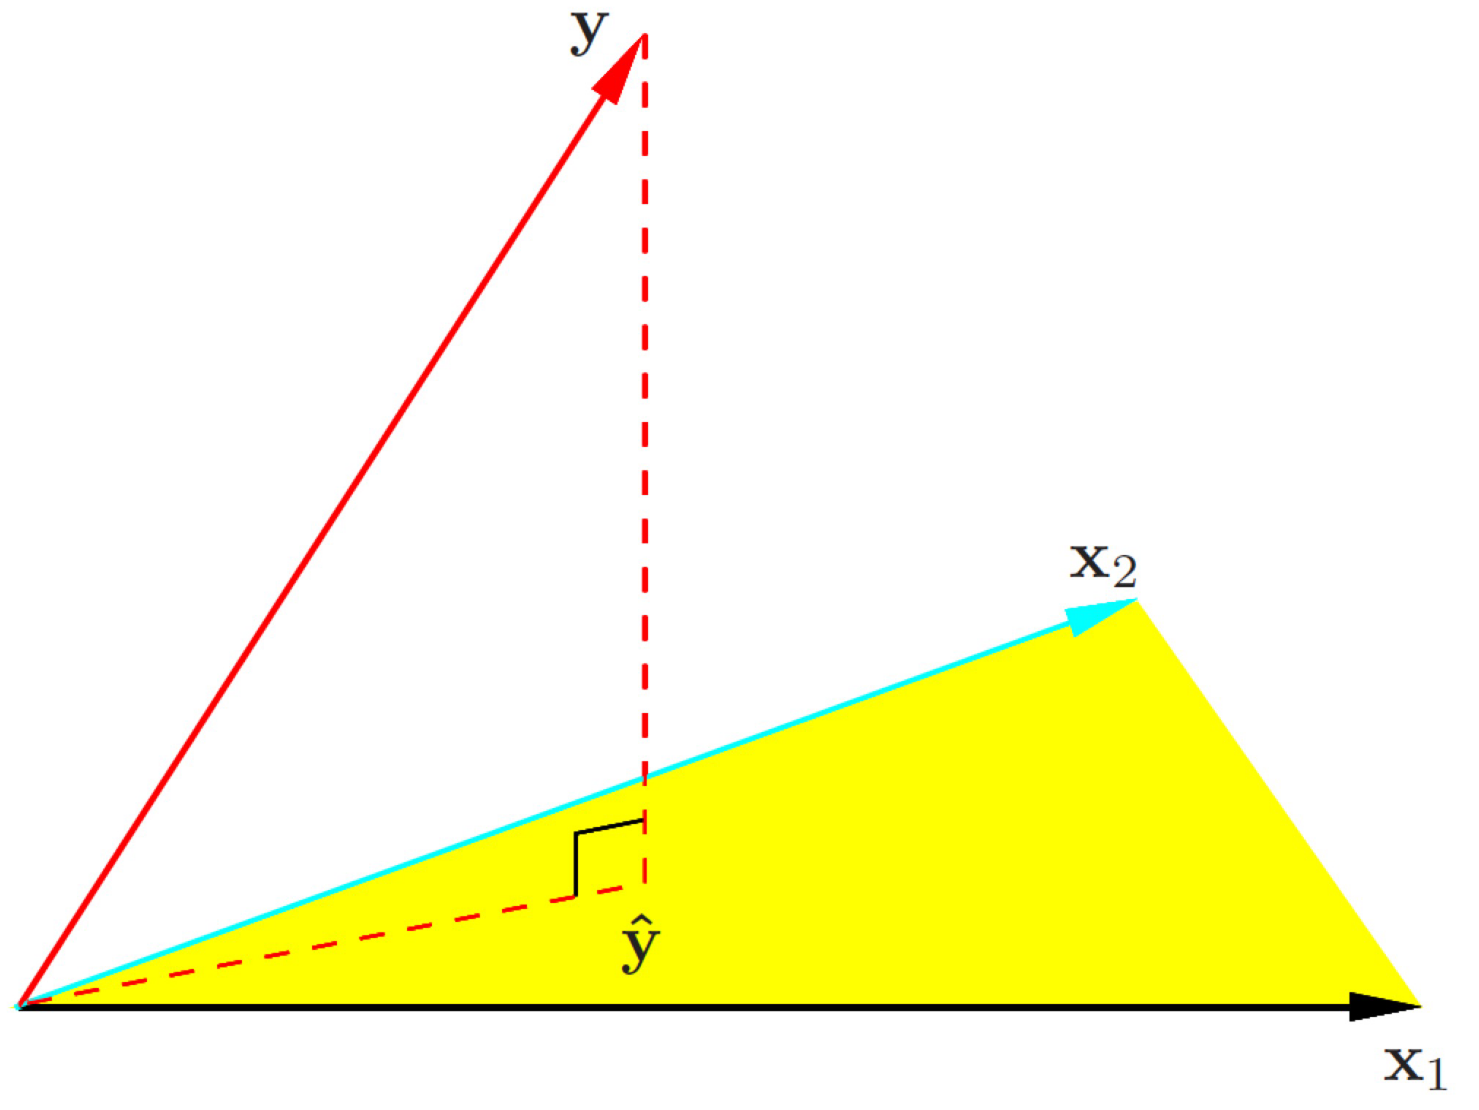
\includegraphics[scale=0.1]{Images/img9.png}
\end{center}

\begin{thmbox}
    \begin{theorem}
        Define residual vector as $r$. Then
        $$r=y-\hat{y}=0.$$
    \end{theorem}
    \begin{prfbox}
        \begin{proof}
            We want to prove that $r\perp X$. Then we wish to prove $X\T r=0$.
            Since:
            \begin{eqnarray*}
                X\T r &=& X\T (y-X\hat{\beta}) \\
                &=& X\T y - X\T X (X\T X)^{-1} X\T y\\
                &=& 0,
            \end{eqnarray*}
            thus $r\perp X$.
        \end{proof}
    \end{prfbox}
\end{thmbox} 

\begin{thmbox}
    \begin{theorem}
        Given the following assumption:

        \begin{itemize}
            \medskip
            \item $y=X\beta+\ve$ (Model Assumption) (i.e. Assume the ground truth model is a linear model.)
            \medskip
            \item $\ve$ is independent of $X$. Moreover, $\ev[\ve_i]=0$
            \medskip
            \item Cov$(\ve_i, \ve_i')=0$ and $\var(\ve_i)=\sigma_e^2$. i.e. $\var(\ve)=\sigma_e^2I$
        \end{itemize}
        \medskip
        Define $\hat{\beta}=(X\T X)^{-1}X\T y$. Then $\hat\beta$ is a unbiased estimator of $\beta$.
        Moreover, $\var(\hat\beta)\sigma_e^2 = (X\T X)^{-1}$ is a square matrix of dimension $(p,p) \text{, or } (p+1,p+1)$ if $\bt{0}$ is in consideration.
    \end{theorem}
\end{thmbox} 



\begin{thmbox}
    \begin{prfbox}
        \begin{proof}
            \begin{eqnarray*}
                \ev(\hat\beta) &=& \ev\bigl[(X\T X)^{-1}X\T y\bigr]\\
                               &=& (X\T X)^{-1}X\T\ev(y) \footnote[1]{$X$\text{ is already observed and is no longer random.}}\\
                               &=& (X\T X)^{-1}X\T X\beta \footnote[2]{$y=X\beta+\ve\implies \ev(y)=\ev(X\beta+\ve)=X\beta$}\\
                               &=& \beta
            \end{eqnarray*}
            \begin{eqnarray*}
                \var(\hat\beta) &=& \var\bigl[(X\T X)^{-1}X\T (X\beta+\ve)\bigr]\\
                                &=& \var\bigl[\beta+(X\T X)^{-1}X\T\ve\bigr]\\
                                &=& \ev\bigl[(X\T X)^{-1}X\T\ve\ve\T X(X\T X)^{-1}\bigr] - \ev\bigl[(X\T X)^{-1}X\T\ve\bigr]\ev\T\bigl[(X\T X)^{-1}X\T \ve\bigr]\\
                                &=& (X\T X)^{-1}X\T\ev(\ve\ve\T)(X\T X)^{-1}X - (X\T X)^{-1}X\T\ev(\ve)\ev\T(\ve)X(X\T X)^{-1}\\
                                &=& X(X\T X)^{-1}X\T\bigl[\underbrace{\ev(\ve\ve\T) - \ev(\ve)\ev\T(\ve)}_{\var(\ve)}\bigr]X(X\T X)^{-1}\\
                                &=& X(X\T X)^{-1}X\T \sigma_e^2 I X(X\T X)^{-1}\\
                                &=& \sigma_e^2 (X\T X)^{-1}
            \end{eqnarray*}
            \begin{notebox}
                \begin{note}
                    The reason why we can directly treat $\var(\ve)$ as $\sigma_e^2 I$, is because of the design of covariance matrix along with the assumption.
                    Note that this matrix has a form of:
                        \[
                            \NiceMatrixOptions{code-for-first-row=\scriptstyle,code-for-last-row=\scriptstyle}
                            \begin{pNiceMatrix}[first-row,first-col]
                                  & \ve_1 & \ve_2 & \cdots & \ve_n\\
                                \ve_1 & \var(\ve_1) & \cov(\ve_1,\ve_2) & \cdots & \cov(\ve_1,\ve_n) \\
                                \ve_2 & \cov(\ve_2,\ve_1) & \var(\ve_2) & \cdots & \cov(\ve_2,\ve_n) \\
                                \vdots & \vdots & 	\vdots & \ddots & \vdots \\
                                \ve_n & \cov(\ve_n,\ve_1) & \cdots & \cdots & \var(\ve_n)\\
                            \end{pNiceMatrix}.
                        \]
                        Since $\cov(\ve_i,\ve_i')$ is 0, thus the matrix is a diagonal matrix. 
                \end{note}
            \end{notebox}
        \end{proof}
    \end{prfbox}
    \begin{notebox}
        \begin{note}
            The model is useful for prediction, even if the assumption is not met, since by bias-variance tradeoff, even if there is bias, but
            due to the simpliness in the model, the variance will be small.
            However, the assumption is critical, if you are doing statistical inference.
        \end{note}
    \end{notebox}
\end{thmbox} 

\subsection{Maximum Likelihood Estimate} \label{MLE}

Assume we have a probablistic model $P(\D|\theta)$, where $\theta$ is the parameter for the probablistic model. 
We know that if we are given the parameters, we can generate data $\D$ from the probablistic model. 

Now, if we are given the observed data $\D$, how can we estimate $\theta$?

Let's take an very simple example: Suppose we have a dataset $\D=\bigl\{z_1,z_2,\cdots, z_n \bigr\}$, where $z_i\sim N(\mu,1)$, and indeed $\theta=\bigl\{ \mu \bigr\}$.

What we wish is to evaluate for:
$$\hat\theta = \arg\max_\theta \log P(\D|\theta).$$

Note the probablistic model for $Z$ is given by:
$$P(z_i|\theta)=\frac{1}{\sqrt{2\pi}}\exp\Biggl(-\frac{1}{2}(z_i-\mu)^2\Biggr).$$

Since for each $z_i$, they are IID (Independent and Identically Distributed), thus: 
$$P(\D|\theta)=\prod_{i=1}^n P(z_i|\theta).$$

Now we take $\log$ on both sides. We now have:

\begin{eqnarray*}
    \log P(\D|\theta)&=&\sum_{i=1}^n \log P(z_i|\theta)\\
                     &=&n\log\Biggl(\frac{1}{\sqrt{2\pi}}\Biggr) + \sum_{i=1}^n -\frac{1}{2}(z_i-\mu)^2.
\end{eqnarray*}

Maximize with respect to $\theta$ on L.H.S. is now equivalent to maximizing with respect to $\mu$ on R.H.S.. So we take derivative on the R.H.S. with respect to $\mu$.
$$\frac{\partial}{\partial\mu} =  \sum_{i=1}^n (z_i-\mu).$$

Set the derivative to be 0, we have:
$$\hat\mu=\frac{1}{n}\sum_{i=1}^n z_i.$$

Now, we apply the concept to linear regression model.

Suppose we are given the data $\D=\Bigl\{(x_i,y_i)\Bigr\}$, where $y_i=x_i\T\beta+\ve_i$ (Sample version, different from the one we previously seen).

Assume that $\ve_i\sim N(0,\sigma_e^2)$. Then we have:
$$\ve_i=y_i-x_i\T\beta\sim N(0,\sigma_e^2).$$

Thus:
$$P(y_i|x_i;\beta)=\frac{1}{\sqrt{2\pi\sigma_e^2}}\exp\Biggl(-\frac{1}{2\sigma_e^2}(y_i-x_i\T\beta)^2\Biggr),$$
and:
$$P(y_i|x;\beta)=\prod_{i=1}^{n}P(y_i|x_i;\beta).$$

We take $\log$ on both sides, and maximize both side w.r.t. $\beta$.
\begin{eqnarray*}
    \hat\beta=\max_\beta\log P(y_i|x;\beta)&=&\max_\beta\Biggl\{\frac{n}{\sqrt{2\pi\sigma_e^2}} + \sum_{i=1}^{n}-\frac{1}{2\sigma_e^2} (y_i-x_i\T\beta)^2\Biggr\}\\
    &=&\max_\beta\sum_{i=1}^{n} (y_i-x_i\T\beta)^2.
\end{eqnarray*}

In the end, since $\ve$ is a constant, maximizing the L.H.S. is actually equivalent to minimizing the sum of ordinary least square.
Thus, the solution for using MLE approach is equivalent to using OLS approach. i.e. $$\hat\beta=(X\T X)^{-1}X\T y.$$

\begin{notebox}
    \begin{note}[Fisher Information Matrix]
        Define $\mathcal{I}$ as the Fisher Information Matrix, where: $$\mathcal{I}=\frac{\partial^2 (\log P(y_i|x;\beta))}{\partial\beta\partial\beta\T}.$$
        Note that if we take inverse to $\mathcal{I}$, we get exactly $\var(\hat\beta)$. This is another method for you to find the variance.
    \end{note}
\end{notebox}

\subsection{Prediction}

Suppose we already have the estimate, $\hat\beta$, and a new data $x_{\text{new}}$. The prediction $y_{\text{new}}$ can be formed by:
    $$\hat{y}_{\text{new}}=x_{\text{new}}\T\hat\beta$$
This is known as point prediction. 
However, we do not sure how accurate our prediction is. 
That is, we do not have an range for the variance of such prediction $\hat{y_{\text{new}}}$.

\begin{thmbox}
    \begin{theorem}
        $$\var(\hat{y}_{\text{new}}) = \var({x}_{\text{new}}\T\hat\beta)$$
    \end{theorem}
    \begin{prfbox}
        \begin{proof}
            Note that:
        \begin{eqnarray*}
            \var(\hat{y}_{\text{new}}) &=& \var({x}_{\text{new}}\T\hat\beta)\\
                                    &=& \ev({x}_{\text{new}}\T\hat\beta\hat\beta\T {x}_{\text{new}}) - \ev({x}_{\text{new}}\T\hat\beta)\ev\T({x}_{\text{new}}\T\hat\beta)\\
                                    &=& {x}_{\text{new}}\T \underbrace{\Biggl[\ev(\hat\beta\hat\beta\T) - \ev(\hat\beta)\ev\T(\hat\beta)\Biggr]}_{\var(\hat\beta)} {x}_{\text{new}}\\
                                    &=& {x}_{\text{new}}\T\var(\hat\beta){x}_{\text{new}}.
        \end{eqnarray*}

        \end{proof}
    \end{prfbox}
\end{thmbox}


\begin{center}
    \begin{tikzpicture}
        % Draw axes
        \draw[->] (0,0) -- (0,4) node[above] {$Y$-axis};
        \draw[->] (0,0) -- (5,0) node[right] {$X$-axis};
    
        % Point estimation
        \draw[fill=red] (2,2.5) circle (2pt) ;
        \draw[fill=red] (3,3) circle (2pt) ;
    
        % Confidence interval bar
        \draw[thick, blue] (2,2) -- (2,3) ;
        \draw[thick, blue] (3,2.5) -- (3,3.5) ;
    
        % Confidence interval ends
        \draw[thick, orange] (1.8,2) -- (2.2,2);
        \draw[thick, orange] (1.8,3) -- (2.2,3);
        \draw[thick, orange] (2.8,2.5) -- (3.2,2.5);
        \draw[thick, orange] (2.8,3.5) -- (3.2,3.5);
    
    \end{tikzpicture}    
\end{center}

The blue bar is also known as the confidence interval. However, in practice, there will be additional noise $\ve_i$.
Thus the predictive interval refers to $$\var(\hat{y_i})+\var(\ve_i)$$.

\subsection{Extension of Linear Model}

Suppose we have a model:
$$Y=\bt{0}+\bt{1}X_1+...+\bt{j}X_j.$$

We can treat each $\bt{i}X_i$ as $f_i(X_i)$. And the formula can be generalized by:
$$Y=\sum_j f_j(X_j).$$

Note that $f_i$ can be some nonlinear function, say you can let $f_1\mapsto 3X_1-4\sin(X_1)$. Then we call such model additive model. 
However, the model $Y=2+\sin(X_1X_2)+X_3$ is not additive.

Another possible generalization is we try to include some interaction / synergy terms.

For example, consider the following model:
$$Y=\bt{0}+\bt{1}X_1+\bt{2}X_2+\bt{3}X_1X_2.$$

Then the interaction term is $\bt{3}X_1X_2$. And it means the effect of $X_1$ on $Y$ depends on $X_2$.

We can also consider some kind of "non-linear model" if the linear model is not good enough. Say:
$$Y=\bt{0}+\bt{1}X+\bt{2}X^2.$$

Note that since $X^2$ is given, thus it is still a linear regression model. OLS methods can still be used to solve the problem.

\subsection{Model Diagnosis}

\subsubsection{Nonlinearity of Data}

In usual cases, we assume our model is a linear model. However, what if the model is not linear?

Suppose we have an observed data $y_i=x_i\T\beta+\ve_i$, and a fitted value $\hat{y}_i=x_i\T\hat\beta$, where $\hat\beta$ is the fitted OLS value. 
Then the residual is defined as $r=y_i-\hat{y}_i$. 

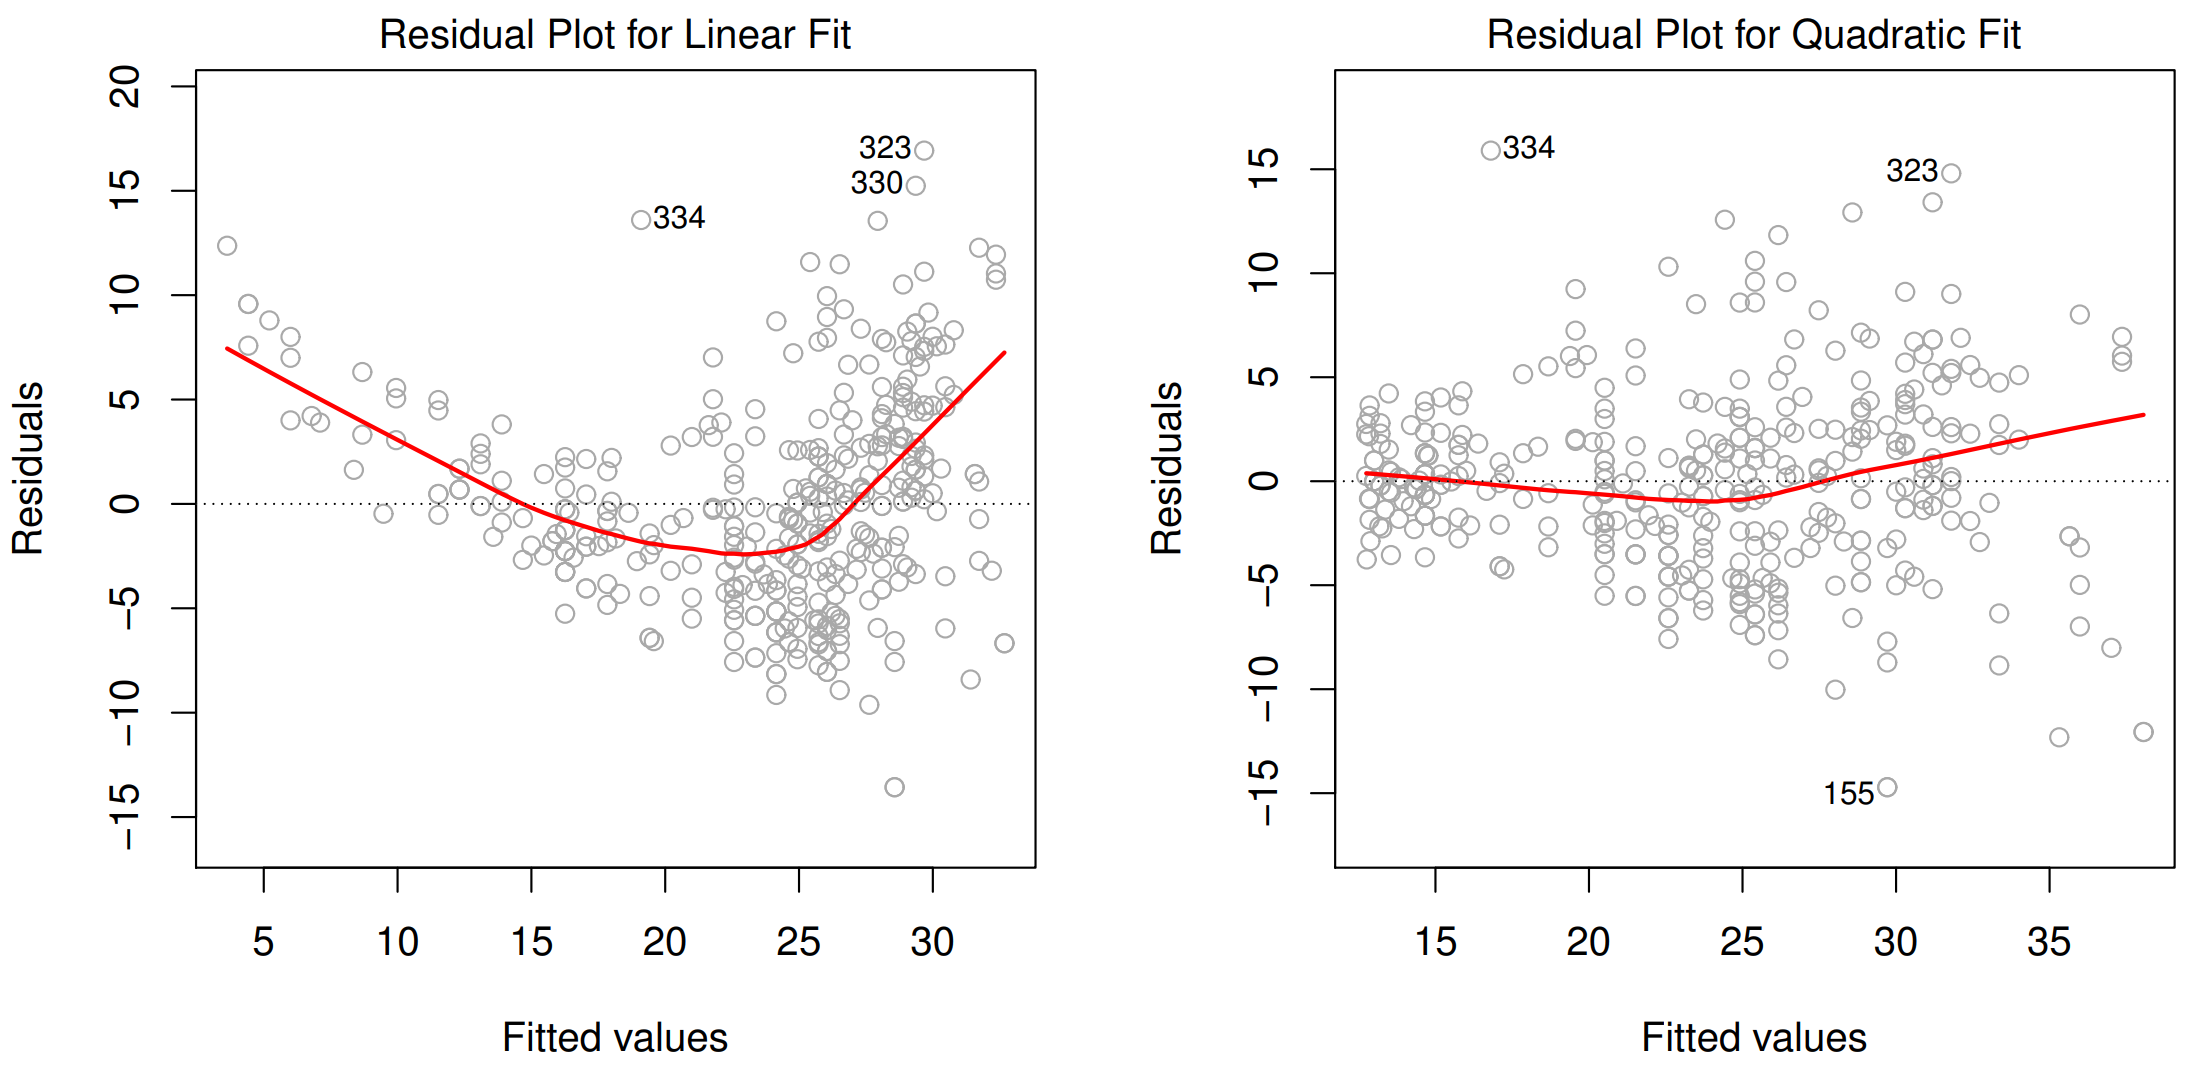
\includegraphics[scale=0.2]{Images/img10.png}

Notice that by our assumption, $\var(\ve_i)=\sigma^2$ is a constant and $\ev(\ve_i)=0$. 
This implies if the residual value is not close to zero and the variance of the residual is varying, then the model must have something wrong (Left one).

To prevent the issue, consider adding nonlinear terms (Right one).

\subsubsection{Correlation of Error Terms}

Previously, we assumed that $\cov(\ve_i,ve_i')=0$. 
If the assumption does not hold, then we will get an incorrect $\var(\hat\beta)$, which will affect the further inferences and testings.

\subsubsection{Non-constant Variance of Error Terms}

We assumed that $\var(\ve_i)=\sigma^2$ is a constant. The model will not be good if the variance in $\var(\ve_i)$ is large. 
One way to detect is by residual graph. 

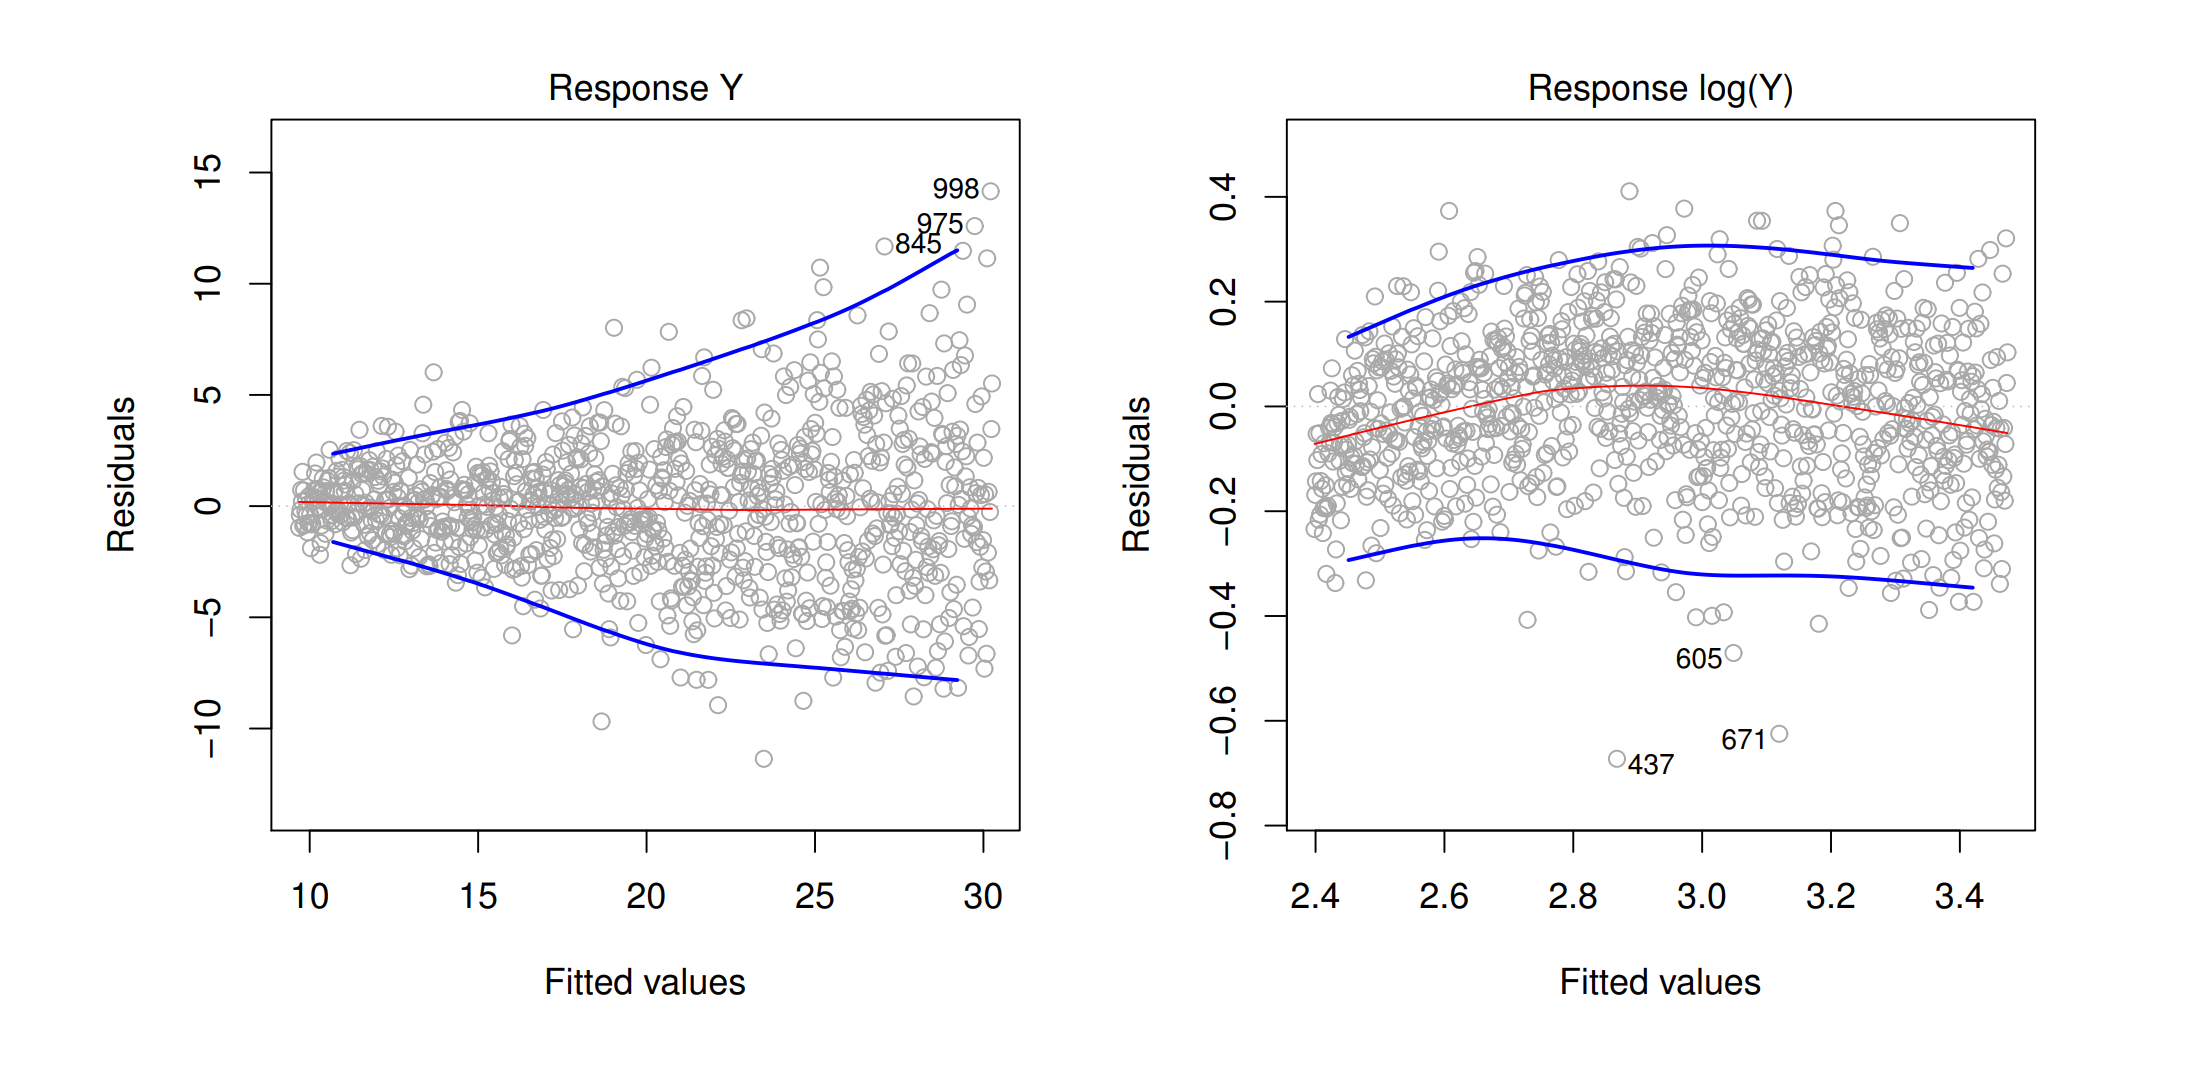
\includegraphics[scale=0.2]{Images/img11.png}

As you can see from the left hand side, the trend is not a straight line, that is, the variance is not a constant.

To make the variance almost a constant, consider taking $\log$ transformation.

\subsubsection{Outliers}

We have assumed that the noise, $\ve_i$ follows a normal distribution $\mathcal{N}\sim (0,\sigma^2)$.
However, in practice, there is some data points that is extremely deviated from the ground truth model. 
Then you will get a model that is different from the ground truth to minimize the error from the deviated data point by using OLS method.

\begin{center}
    \begin{tikzpicture}

        % Draw axes
        \draw[->] (0,0) -- (10,0) node[right] {$X$};
        \draw[->] (0,0) -- (0,6) node[above] {$Y$};
        
        % Draw ground truth line
        \draw[blue, thick] (0,1) -- (10,5) node[right] {Ground Truth Model};
        
        % Draw data points
        \foreach \x in {1, 2, 3, 4, 5, 6, 7, 8, 9} {
            \pgfmathsetmacro{\y}{0.5*\x + rand*0.5}
            \fill[black] (\x,\y) circle (2pt);
        }
        
        % Draw outlier point
        \fill[red] (5,5) circle (4pt) node[above right] {Outlier};
        
        % Draw adjusted least squares line
        \draw[orange, thick, dashed] (0,2) -- (10,5.5) node[right] {OLS Model (with Outlier)};
        
    \end{tikzpicture}
\end{center}
    
One of the solution is that, we only consider the absolute value of the error term, instead of squared value as used in OLS.
Then the new model will be robust to outliers.

The reason we are not using this model is because the minimization task now becomes:
$$\min_\beta\sum_i|y_i-x_i\T\beta|.$$

And this is not differentiable, and we thus cannot obtain a closed-form solution. 

Another way is to add a weight for different $\beta$. The task now becomes:
$$\min_\beta\sum_{i=1}^nw_i\bigl(y_i-x_i\beta\bigr)^2$$

Intuitively, if there is an outlier, then the weight will be close to 0. The method to determine for $w_i$ is shown as below.

\begin{lstlisting}[ mathescape]
    $w_i \gets 1$
    $\hat\beta\gets(X\T X)^{-1}X\T Y$
    while the algorithm does not converge do:
        $r_i\gets y_i-x_i\T\hat\beta$
        Assign $w_i \gets 1 / r_i^2$
        Evaluate for the OLS with the weight with $\hat\beta\gets (X\T WX)^{-1}X\T WY$.
        Update the weight $w_i$
\end{lstlisting}

\subsubsection{High-leverage Points (and model flexibility)}

It is very difficult to distinguish high-leverage point and outliers visually. Consider the following:

\begin{defbox}
    \begin{definition}[High Leverage Point]
        Let $\mathcal{D}=\bigl\{x_i,y_i\bigr\}$ be the training dataset. Assume that $y_i=x_i\T\beta+\ve_i, i=1\cdots n$.
        Then the ordinary least square solution for $\hat\beta=(X\T X)\inv X\T y$. Then the fitted value of $\hat y=X\hat\beta$, where
        $y=\begin{bmatrix}
            y_1\\
            y_2\\
            \vdots\\
            y_n
            \end{bmatrix}	
        $ is a column vector. Then if $\pd{\hat y_i}{y_i}$, the model sensitivity, is large, then $i$ is said to be a leverage point.
        
    \end{definition}
\end{defbox}

This means that a small change in the $y_i$ will leads to a large change in $\hat y_i$ if such point is high leverage. 

From the equation stated in definition, we have $\hat y=X(X\T X)\inv X\T y$.

\begin{thmbox}
    \begin{theorem}
        Let $H=X(X\T X)\inv X\T$. It is called hat matrix. Then $\pd{\hat y_i}{y_i}=H_{ii}$. 
    \end{theorem}
    \begin{prfbox}
        \begin{proof}
            Given that $\hat y=X(X\T X)\inv X\T y$, and $H=X(X\T X)\inv X\T$, we can rewrite $\hat y=H y$.

            Note that $y$ has a dimension of $(n,1)$. This implies $H$ has a dimension of $(n,n)$. Thus:

            $$
                \begin{bmatrix}
                    \hat y_1\\
                    \hat y_2\\
                    \vdots\\
                    \hat y_n
                \end{bmatrix} = 
                \begin{bmatrix}
                    h_{11} & h_{12} & \cdots & h_{1n}\\
                    h_{21} & h_{12} & \cdots & h_{1n}\\
                    \vdots & \vdots & \ddots & h_{1n}\\
                    h_{n1} & h_{n2} & \cdots & h_{nn}\\
                \end{bmatrix}
                \begin{bmatrix}
                    y_1\\
                    y_2\\
                    \vdots\\
                    y_n
                \end{bmatrix}.
            $$

            Then $\hat y_i=h_{i1}y_1+h_{i2}y_2+\cdots+h_{in}y_n$. The partial derivative $\pd{\hat y_i}{y_i}=h_{ii}$.
        \end{proof}
    \end{prfbox}
\end{thmbox} 


\begin{thmbox}
    \begin{theorem}
        Here are some interesting properties related to $H$. (Just something fun to know, not required)
        \begin{enumerate}
            \item H is a $n\times n$ symmetric matrix.
            \item $H\times H=H$
        \end{enumerate}
    \end{theorem}
    \begin{prfbox}
        \begin{proof}
            Left as exercise to reader.
        \end{proof}
    \end{prfbox}
\end{thmbox} 

From this we can see that high leverage point actually only depends on $X$, while outliers depends on both $X$ and $y$.

Note that a point can be both high leverage point and outlier.

\begin{center}
    \includegraphics*[scale=0.24]{Images/img12.png}
\end{center}

Now, let's consider the sensitivity of all the data points, $\sum_{i=0}^n \pd{\hat y_i}{y_i}$. 

\begin{thmbox}
    \begin{theorem}
        \vphantom{.}

        $\sum_{i=0}^n \pd{\hat y_i}{y_i}=p$, where $p$ is the size of the matrix $X^T X$.
    \end{theorem}
    \begin{prfbox}
        \begin{proof}
            \begin{eqnarray*}
                \sum_{i=0}^n \pd{\hat y_i}{y_i} &=& \sum_{i=0}^n h_{ii}\\
                                                &=& \tr(H)\\
                                                &=& \tr\biggl(X(X\T X)\inv X\T\biggr)
            \end{eqnarray*}
            Since $\tr(AB)=\tr(BA)$, thus
            \begin{eqnarray*}
                \tr\biggl(X(X\T X)\inv X\T\biggr) &=& \tr\biggl((X\T X)\inv X\T X\biggr)\\
                                                  &=& \tr(I_p)\\
                                                  &=& p
            \end{eqnarray*}
        \end{proof}
    \end{prfbox}
\end{thmbox} 

Note that $p$ means the number of parameters. This means the more parameters in the model, the
higher the sensitivity of all the data points.

Let's go back to this image introduced at the beginning.:

\begin{center}
    \includegraphics*[scale=0.3]{Images/img2.png}
\end{center}

Assume that we have the data $\bigl\{(x_i,y_i)\bigr\},i=1\cdots n$, and assume the model is very flexible, say $\hat y_i=\hat f(x_i)=y_i$,
then $\pd{\hat y_i}{y_i}=1$. Summing up, we have $\sum_{i=0}^n \pd{\hat y_i}{y_i}=n$. Note this is the upper bound for the flexibility of the model.

The higher the model flexibility, the more sentitive the model is to a new data point. This implies that whenever a data point changes a little, the model
is able to capture the change and fit into the data point.

Note that one should not simply defines model flexibility as the number of parameters. 
It also depends on how many constraints given to the parameters.

\subsubsection{Collinearity}

Consider the following data:

\begin{center}
    \includegraphics*[scale=0.25]{Images/img13.png}
\end{center}

Note that the two data \texttt{Limit} and \texttt{Rating} are highly correlated. Then these two data exists some collinearity.

From a linear algebra view, let $X$ be a design matrix 
$\begin{bmatrix}
    x_1 & x_2 & \cdots & x_p
\end{bmatrix}$, where each $x_i$ is a column vector. 
Collinearity implies there exist a column that is a linear combination of all other columns.
In other words, the design matrix $X$ is not full rank.

In such situation, we will run into problem, since $X$ is not full rank implies $X\T X$ is not full rank also.
Then $(X\T X)\inv$ does not exist. 

To handle such cases, in the old days we adopt a method, where we want to find out which column is
a linear combination of other columns. We pick the $j$-th column as response $Y$. Then we will regress $Y$ with
other variables. If $R^2$ is close to 1, then this implies that this variable can be represented by other variables 
by linear combination. Define inflation vector as:
$$
VIF(\hat\beta_j)=\frac{1}{1-R^2_{X_j|X_{-j}}}
$$

Then the vector will be very large if $R^2$ is close to 1.

In nowadays, we will solve by slightly modifying the ordinary least square solution like this:
$$
\hat\beta=(X\T X+\lambda I)\inv X\T y,
$$

where $\lambda$ is a positive constant, and $I$ is the identity matrix. This is what we called Ridge regression. We will study this part deeply later.

The following parts (Hypothesis testing) will not be included in the final exam but can be used as a reference.

\subsubsection{Hypothesis testing of OLS (Not included in final)}

Given that $\hat\beta=(X\T X)\inv X\T y$, and the three assumption stated in the earlier times, we have:

$$
\begin{cases}
\ev(\hat\beta)=\beta \\
\var(\hat\beta)=\sigma^2(X\T X)\inv
\end{cases}
$$

Consider the $j$-th variable $\hat\beta_j$. Define $t=\frac{\hat\beta_j}{\hat\sigma_j}$.
View $\hat\beta$ as a random variable, then by central limit theorem, $\hat\beta\sim \mathcal{N}(\beta,\sigma^2(X\T X))$. Then we have $\hat\beta-\beta\sim\mathcal{N}(0,\sigma^2(X\T X))$.

It follows that for the $j$-th variable, we have $\hat\beta_j-\beta_j\sim\mathcal{N}(0,\sigma^2_j)$. Then $\frac{\hat\beta_j-\beta_j}{\sigma_j}\sim\mathcal{N}(0,1)$.

We define our null hypothesis to be $H_0:\beta_j=0$. 
The reason we want to test this is because we want to see if $Y=\sum_jX_J\beta_j+\ve=0$.
Assume the hypothesis is true / hold. If the observed data is consistent, then the hypothesis is very likely to be true. 

If the hypothesis holds, then $z_j=\frac{\hat\beta_j}{\hat\sigma_j}\sim \mathcal{N}(0,1)$. The value is called $z$-value, and $\mathcal{N}(0,1)$ is called null distribution.

\begin{center}
    \begin{tikzpicture}
        \begin{axis}[
            axis lines = middle,
            xlabel = $x$,
            ylabel = {$f(x)$},
            xtick={-3,-2,-1,0,1,2,3},
            ytick={0,0.1,0.2,0.3},
            ymin=0, ymax=0.4,
            samples=100,
            domain=-4:4,
            enlargelimits,
            grid = both,
            title={Normal Distribution ($\mu=0$, $\sigma=1$)},
            ]
            \addplot[blue, thick] {1/(sqrt(2*pi))*exp(-x^2/2)};
    
            % Points
            \addplot[red, only marks, mark=*] coordinates {(1,0)};
            \addplot[orange, only marks, mark=*] coordinates {(4.5,0)};
    
        \end{axis}
    \end{tikzpicture}
\end{center}

Suppose the test statistic $z_j$ lies in the red point, then the evidence is not contradictory to the null distribution. 
However, if the observation lies in the orange point, then the evidence is contradictory to the distribution. To test for the 
evidence, we introduce the concept called $p$-value. $p$-value is defined as:
$$
P(|z|>z_{obs}|H_0 \text{ holds})
$$

\begin{center}
    \begin{tikzpicture}
        \begin{axis}[
            axis lines = middle,
            xlabel = $x$,
            ylabel = {$f(x)$},
            xtick={-3,-2,-1,0,1,2,3},
            ytick={0,0.1,0.2,0.3},
            ymin=0, ymax=0.4,
            samples=100,
            domain=-4:4,
            enlargelimits,
            grid = both,
            title={Normal Distribution ($\mu=0$, $\sigma=1$)},
            ]
            % Plot the normal distribution
            \addplot[blue, thick] {1/(sqrt(2*pi))*exp(-x^2/2)};
    
            % Shade the area to the right of x=1
            \addplot [
                domain=1:4, 
                samples=50, 
                fill=red, 
                opacity=0.5
            ] {1/(sqrt(2*pi))*exp(-x^2/2)} \closedcycle;
    
            % Point at (1,0)
            \addplot[red, only marks, mark=*] coordinates {(1,0)};
    
            % P-value label
            \node at (axis cs:3,0.15) [anchor=north] {$p$-value area};
        \end{axis}
    \end{tikzpicture}
\end{center}

If $p$-value is greater than a specific value, then it seems we do not have enough evidence to reject null hypothesis. 
In contrast, if the $p$-value is very small, then the observed data does not follow the distribution. It means we have enough evidence to 
reject the null hypothesis.

Actually, notice that $\hat\sigma_j$ is an estimated value, thus we actually need to use $t$-distribution instead of normal distribution.

\subsection{K-Nearest Neighbours (KNN)}

Suppose we have the training data $\mathcal{D}=\bigl\{(x_i,y_i)\bigr\}$, where $x_i\in\mathbb{R}^p$, while $y_i\in\mathbb{R}$.
Given any query point $x_0$, we are going to find the nearest neighbour $N(x_0)$ of the query point based on the number of $K$.

\begin{center}
    \begin{tikzpicture}

        % Draw x-y axis
        \draw[->] (-1,0) -- (6,0) node[right] {$x_1$};
        \draw[->] (0,-1) -- (0,6) node[above] {$x_2$};
        
        % Draw blue data points
        \fill[blue] (1,1) circle (3pt);
        \fill[blue] (2,3) circle (3pt);
        \fill[blue] (3,2) circle (3pt);
        \fill[blue] (4,4) circle (3pt);
        \fill[blue] (5,1) circle (3pt);
        \fill[blue] (5,5) circle (3pt);
        \fill[blue] (1,5) circle (3pt);
        \fill[blue] (-1,3) circle (3pt);


        % Draw the query point in red
        \fill[red] (3,3) circle (3pt);
        
        % Highlight the 3 nearest neighbours in orange
        \fill[orange] (2,3) circle (3pt);
        \fill[orange] (3,2) circle (3pt);
        \fill[orange] (4,4) circle (3pt);
        
    \end{tikzpicture}    
\end{center}

Then $\hat y$ is predicted as:

$$
\hat y=\frac{1}{K}\sum_{i\in N(x_0)}y_i
$$

Instead of using KNN as regression, we may also use KNN as classification, where majority vote method is being used.

\begin{center}
    \includegraphics*[scale=0.4]{Images/img14.png}
\end{center}

The one on the left is $K=1$, while the one on the right is $K=9$. It is easy to observe the curve plotted is smoother when $K$ is large.

\begin{center}
    \includegraphics*[scale=0.4]{Images/img15.png}
\end{center}

This is the 1-D dataset. Indeed KNN is flexible from the plot. Note the black line is the linear model.

\begin{center}
    \includegraphics*[scale=0.2]{Images/img16.png}
\end{center}

Testing error for KNN model. Note that $1/K$ is small implies $K$ is large. Note the error is quite large when compared
with a linear model since the ground truth is actually linear.

\begin{center}
    \includegraphics*[scale=0.2]{Images/img17.png}
\end{center}

Another extreme case, where the data is non-linear in relationship. In this case, KNN is doing better than linear model since linear model
will give a large bias.

\begin{center}
    \includegraphics*[scale=0.2]{Images/img18.png}
\end{center}

This case demonstrates the introduction of noise variables. In the beginning, KNN performs
better than linear model. As the number of noise variable increases, the test error of KNN increases drastically. 

\section{Classification}

Given some training data $\mathcal{D}=\Bigl\{(x_i,y_i)\Bigr\}_{i=1...n}$, where $x_i\in\mathbb{R}^p$, while $y_i\in{0,1}$.
This is called 2-class classification problem.

Consider the following case:

\begin{center}
    \includegraphics*[scale=0.2]{Images/img19.png}
\end{center}

In this case, the linear regression model is not good for classification, since the output is not constrainted between 0 and 1.
This is the reason why we introduce logistic regression.

\subsection{Logistic Regression}

\begin{defbox}
    \begin{definition}[Logistic Regression]
        The logistic regression is defined as: 
        $$
        P(Y=1|X)=\frac{1}{1+\exp(-\beta\T X)}.
        $$
        The probability is indeed bounded between 0 and 1.
    \end{definition}
\end{defbox}

\begin{thmbox}
    \begin{theorem}
        $$
        P(Y=0|X)=\frac{1}{1+\exp(\beta\T X)}.
        $$        
    \end{theorem}
    \begin{prfbox}
        \begin{proof}
            \begin{eqnarray*}
                P(Y=1|X) &=& 1 - P(Y=0|X)\\
                         &=& 1 - \frac{1}{1+\exp(-\beta\T X)}\\
                         &=& \Biggl[\frac{\exp(-\beta\T X)}{1+\exp(-\beta\T X)}\Biggr]\Biggl[\frac{\exp(\beta\T X)}{\exp(\beta\T X)}\Biggr]\\
                         &=& \frac{1}{1+\exp(\beta\T X)}.
            \end{eqnarray*}
        \end{proof}
    \end{prfbox}
\end{thmbox}

\begin{thmbox}
    \begin{theorem}
        $$\log{\frac{P(Y=1|X)}{P(Y=0|X)}}=\beta\T X$$
    \end{theorem}
    \begin{prfbox}
        \begin{proof}
            \begin{eqnarray*}
                \log{\frac{P(Y=1|X)}{P(Y=0|X)}} &=& \log{\Biggl[\frac{1}{1+\exp(-\beta\T X)}\Biggr]\Biggl[\frac{1+\exp(-\beta\T X)}{\exp(-\beta\T X)}\Biggr]}\\
                                                &=& \log{\Biggl[\frac{1}{\exp(-\beta\T X)}\Biggr]}\\
                                                &=& \beta\T X
            \end{eqnarray*}
        \end{proof}
    \end{prfbox}
    This is called log-odds ratio.
\end{thmbox}

Let's go back to a polulational linear model, where $Y=X\T\beta+\ve$, or $Y=\beta\T X+\ve$. Suppose that $\ve$ is zero mean, then $\ev(Y\vert X)=\beta\T X$.

Since the log-odds scale is also linear, this implies we can generalize on the non-linear function. Details will be given later.

We will explain on how to perform parametric estimation for $\beta$ on the log-odds scale. 
Notice that the ordinary least square solution that we used on linear regression no longer applies.
For log-odds ratio we do not have a closed form solution. 

We will do the same thing for logistic regression as what we did in linear regression. Click \ref{MLE} as a reference.

\begin{notebox}
    \begin{note}
        The derivation below may have skipped some proof for the pace concern. I think I will put the proof back after Winter.
    \end{note}
\end{notebox}

By definition, we have $P(Y=1|X)=\frac{1}{1+\exp(-\beta\T X)}.$ Assume that for the given $x_i$, all the $y_i$ are independent, then we can rewrite the probability
density function as:
\begin{eqnarray*}
    P(y\vert X,\beta) &=& \prod_{i=1}^n P(y_i\vert x_i;\beta)\\
                      &=& \prod_{i:y_i=0}P(y_i=1\vert x_i;\beta) \prod_{i:y_i=1}^nP(y_i=0\vert x_i;\beta)\\
                      &=& \prod_{i:y_i=0}\frac{1}{1+\exp(-\beta\T x_i)} \prod_{i:y_i=1}^n\frac{1}{1+\exp(\beta\T x_i)}\\
                      &\overset{\text{equiv.}}{=}& \prod_{i:y_i=0}\frac{\exp(y_i\beta\T x_i)}{1+\exp(\beta\T x_i)}\\
    l=\log P(y\vert X,\beta) &=& \sum_{i=1}^n \Bigl[y_i\beta\T x_i-\log(1+\exp(\beta\T x_i))\Bigr]
\end{eqnarray*}

Since there is no closed form solution for $\nabla l$, or $\pd{l}{\beta}$,
we will use Newton's method to perform maximum likelihood approach. Here is the idea (For single variable calculus).

Suppose we want to find $x$, such that 
$$
    g(x) = \frac{\dd{f}}{\dd{x}} = 0.
$$
Assume that $x_0$ is one of the solution for the equation. Then we perform first-order linear approximation with:
$$
    g(x)\simeq g(x_0)+g'(x_0)(x-x_0).
$$
Then $x$ is given by:
$$
    x = x_0-g(x_0)\bigl[g'(x_0)\bigr]\inv.
$$

We will perform the operation again and again, with each $x_0$ the $x$ evaluated at the previous estimations.

Now, let's come back to our problem, that we want to solve for $g(\beta)=\pd{l}{\beta}=0$.

Then by Newton's method, we have:
$$
    \beta_{\text{new}} = \beta_{\text{old}}-g(\beta_{\text{old}})\bigl[g'(\beta_{\text{old}})\bigr]\inv.
$$
We will need to evaluate for the gradient, $g(\beta_{\text{old}})$, and Hessian matrix $\bigl[g'(\beta_{\text{old}})\bigr]$ to evaluate for the new point.
Recall the likelihood formula:
$$
    l(\beta)=\log P(y\vert X,\beta) = \sum_{i=1}^n \Bigl[y_i\beta\T x_i-\log(1+\exp(\beta\T x_i))\Bigr].
$$
We now take the first order derivative to $l$.
\begin{eqnarray*}
    \pd{l}{\beta} &=& \sum_{i=1}^n \Biggl[y_ix_i-\frac{\exp(\beta\T x_i)x_i}{1+\exp(\beta\T x_i)}\Biggr]\\
                  &=& \sum_{i=1}^n \Biggl[y_i-\frac{1}{1+\exp(-\beta\T x_i)}\Biggr]x_i.
\end{eqnarray*}
Note that $\frac{1}{1+\exp(-\beta\T x_i)}$ is exactly the same as $P(Y=1\vert X=x_i)$. We give it a name $P_i$ for simplicity. Then,
$$
\pd{l}{\beta} = \sum_{i=1}^n \bigl(y_i-P_i\bigr)x_i
$$
It is easy to show that $ \sum_{i=1}^n \bigl(y_i-P_i\bigr)x_i = X\T (y-P)$. This is left as an exercise to reader. (Remind me to put the proof on my site if I have time since space here is not sufficient.)

Now, we can tell why there is no closed form solution of $\nabla l$ is because the derivative involves summation and the parameter we wish to estimate.
It will be extremely difficult for us to evaluate for a closed form solution.

Let's come back to $\pd{l}{\beta}$. We want to calculate for the second derivative. Recall that:
$$
\pd{l}{\beta} =\sum_{i=1}^n \Biggl[y_i-\frac{1}{1+\exp(-\beta\T x_i)}\Biggr]x_i.
$$
Taking the derivative again, we have:
\begin{eqnarray*}
    \pd{}{\beta\T} &=& \pd{}{\beta\T}\sum_{i=1}^n \Biggl[y_i-\frac{1}{1+\exp(-\beta\T x_i)}\Biggr]x_i\\
                   &=& \sum_{i=1}^n x_i\Biggl[-\frac{\exp(-\beta\T x_i)(-x_i\T)}{(1+\exp(-\beta\T x_i))^2}\Biggr]\\
                   &=& -\sum_{i=1}^n x_i \Biggl[\frac{1}{(1+\exp(-\beta\T x_i))}\Biggr]\Biggl[\frac{\exp(-\beta\T x_i)}{(1+\exp(-\beta\T x_i))}\Biggr]x_i\T\\
                   &=& -\sum_{i=1}^n x_i P_i (1-P_i) x_i\T\\
                   &=& -\sum_{i=1}^n P_i (1-P_i) x_i x_i\T.
\end{eqnarray*}

This is in fact the Hessian matrix, and it can further be rewritten as $-x\T Wx$,

where $W=\text{diag}(P_1 (1-P_1),...,P_n (1-P_n))$ is a diagonal matrix.

To perform Newton's method, we first initiallize $\beta_{\text{old}}$ as a zero vector. Then: 
\begin{eqnarray*}
    \beta_{\text{new}} &=& \beta_{\text{old}} - H\inv\vert_{\beta_{\text{old}}} g\vert_{\beta_{\text{old}}}\\
                       &=& \beta_{\text{old}} + (x\T Wx)\inv x\T(y-p)\\
                       &=& (x\T Wx)\inv x\T Wz,
\end{eqnarray*}
where $z=\beta_{\text{old}}+w\inv(y-p)$

The reason why we separate $z$ out, is because it can be viewed as iterative reweighted least square form.

[2024-10-10 END]

\newpage
remarks for smoking: below notes start from p.35 of lecture3.pdf 
\begin{defbox}
    \begin{definition}[Confusion matrix]

        Define the confusion matrix as:

        \[
            \NiceMatrixOptions{code-for-first-row=\scriptstyle,code-for-last-row=\scriptstyle}
            \begin{pNiceMatrix}[first-row,first-col]
                  & +ve & -ve \\
                +ve & TP  & FN \\
                -ve & FP & TN  \\
            \end{pNiceMatrix}.
        \]


        where:

        \begin{itemize}
            \item         True Positive(TP): Predicted is \textbf{positive(1)}, and the truth is \textbf{positive(1)}
             
            \item         False Positive(FP): Predicted is \textbf{positive(1)}, but the truth is \textbf{negative(0)}
             
            \item         True Negative(TN):  Predicted is \textbf{negative(0)}, and the truth is \textbf{negative(0)} 
           
            \item         False Negative(FN): Predicted is \textbf{negative(0)}, but the truth is \textbf{positive(1)}        
        \end{itemize}




    \end{definition}
\end{defbox}

some terminology of Confusion matrix:
\begin{defbox}
    \begin{definition}[sensitivity]
        \begin{itemize}
            below are things equivalent to sensitivity:
            \item $\textbf{Positive True Rate}$
            \item $P(\hat{y_i} = 1 \mid y_i = 1)$
            \item $\frac{TP}{TP + FN}$
        \end{itemize}
    \end{definition}
\end{defbox}

\begin{defbox}
    \begin{definition}[specificity]
        \begin{itemize}
            below are things equivalent to specificity:
            \item $\textbf{Negative True Rate}$
            \item $P(\hat{y_i} = 0 \mid y_i = 0)$
            \item $\frac{TN}{FP + TN}$
        \end{itemize}
    \end{definition}
\end{defbox}

\begin{defbox}
    \begin{definition}[Type I error]
        \begin{itemize}
            below are things equivalent to Type I error:
            \item $\textbf{Positive False Rate}$
            \item $P(\hat{y_i} = 1 \mid y_i = 0)$
            \item $\frac{FP}{FP + TN}$
        \end{itemize}
    \end{definition}
\end{defbox}

\begin{defbox}
    \begin{definition}[Type II error]
        \begin{itemize}
            below are things equivalent to Type II error:
            \item $\textbf{Negative False Rate}$
            \item $P(\hat{y_i} = 0 \mid y_i = 1)$
            \item $\frac{FN}{TP + FN}$
        \end{itemize}
    \end{definition}
\end{defbox}


\end{document}

% Below are some boxes that may help with your document. They are not rendered during compilation.

% Definition
\begin{defbox}
    \begin{definition}[]

    \end{definition}
\end{defbox}

% Theorem (With a proof box included, remove if necessary)
\begin{thmbox}
    \begin{theorem}

    \end{theorem}
    \begin{prfbox}
        \begin{proof}
            
        \end{proof}
    \end{prfbox}
\end{thmbox} 

% Example
\begin{expbox}
    \begin{example}

    \end{example}
\end{expbox}

% Warning / Remarks
\begin{warnbox}
    \begin{warning}

    \end{warning}
\end{warnbox}

\begin{warnbox}
    \begin{remark}

    \end{remark}
\end{warnbox}

% Notes
\begin{notebox}
    \begin{note}

    \end{note}
\end{notebox}